\documentclass{ieeeaccess}
\usepackage{cite}
% Slightly tighter float-to-text separation (within IEEE norms); content and float placement are unchanged.
\setlength{\textfloatsep}{13pt plus 2pt minus 4pt}
\setlength{\dbltextfloatsep}{13pt plus 2pt minus 4pt}
\usepackage{url}
% Allow URL line breaks at common URL separators to prevent overflow
\makeatletter
\g@addto@macro\UrlBreaks{\do\/\do\-\do\.\do\_\do\?\do\&\do\=\do\#\do\:}
\makeatother
\usepackage{amsmath,amssymb,amsfonts}
\usepackage{algorithmic}
\usepackage{graphicx}
\usepackage{textcomp}
\usepackage{booktabs}

% --- Revision marking (Access-2026-34370 resubmission) -----------------------
% Every change relative to the submitted version is wrapped in \revised{...}.
% \highlighttrue  -> changed text set in blue (intermediate build); the
%                    "Highlighted PDF" is derived from it (black text, yellow highlight)
% \highlightfalse -> text in the surrounding colour ("Main Manuscript", clean build);
%                    the clean branch keeps a colour group so that line and page
%                    breaking are identical in the two builds
\usepackage{xcolor}
\newif\ifhighlight \highlightfalse
% URLs changed in this revision, defined verbatim so that they can be highlighted by \revised
\urldef{\urlocpp}\url{https://openchargealliance.org/protocols/open-charge-point-protocol/}
\urldef{\urlabb}\url{https://library.e.abb.com/public/8f07987a3a284da6bf4e4f8f53cd6502/ABB_Terra_AC_Charger_OCPP1.6_ImplementationOverview%20_v1.8_FW1.6.6.pdf}
\urldef{\urlrepo}\url{https://github.com/SmartGridLab/Posterior-Aware-Online-Matching-of-EV-Charger-Pairs-under-Delayed-Anonymous-Telemetry}
\DeclareRobustCommand{\revised}[1]{\ifhighlight{\color{blue}#1}\else{\color{.}#1}\fi}
% ------------------------------------------------------------------------------

% Relax float placement to keep figures near their citations
\renewcommand{\topfraction}{0.95}
\renewcommand{\bottomfraction}{0.8}
\renewcommand{\textfraction}{0.05}
\renewcommand{\floatpagefraction}{0.6}
\renewcommand{\dbltopfraction}{0.95}
\renewcommand{\dblfloatpagefraction}{0.6}

\def\BibTeX{{\rm B\kern-.05em{\sc i\kern-.025em b}\kern-.08em
T\kern-.1667em\lower.7ex\hbox{E}\kern-.125emX}}

% Override IEEE Access template placeholder for volume/year (class defaults: vol 11, 2023)
\def\thevol{00}
\def\theyear{2026}

\begin{document}
    \history{Date of publication xxxx 00, 0000, date of current version xxxx 00, 0000.}
    \doi{10.1109/ACCESS.XXXXXXXXX}

    \title{\revised{Watermark-Based Online EV--Charger Matching from Delayed Slot-Unlabeled Telemetry}}

    \author{\uppercase{Jiseok Yang}\authorrefmark{1},
        \uppercase{Daisuke Kodaira}\authorrefmark{2}, \IEEEmembership{Member, IEEE}}

    \address[1]{Degree Programs in Systems and Information Engineering, Graduate School of Science and Technology, University of Tsukuba, Tsukuba 305-8573, Japan}
    \address[2]{Institute of Systems and Information Engineering, University of Tsukuba, Tsukuba 305-8573, Japan}

    \tfootnote{This work was supported by the Human Security Collaboration (HSC) Projects, University of Tsukuba, and JSPS KAKENHI Grant Number JP26K01440.}

    \markboth
    {Yang \headeretal: Watermark-Based Online EV--Charger Matching from Delayed Slot-Unlabeled Telemetry}
    {Yang \headeretal: Watermark-Based Online EV--Charger Matching from Delayed Slot-Unlabeled Telemetry}

    \corresp{Corresponding author: Daisuke Kodaira (e-mail: kodaira.daisuke.gf@u.tsukuba.ac.jp).}

                    \begin{abstract}
        \revised{Smart charging and vehicle-to-grid operation require the charging backend to identify the electric vehicle (EV) connected to each charger. However, widely deployed IEC 61851 alternating-current chargers do not convey vehicle identity, leaving EV--charger associations unavailable at multi-port charging sites. Prior current-modulation studies infer these associations by comparing charger-side current commands with vehicle-side current responses, but they assume a static batch of simultaneous sessions with complete waveforms. Accordingly, this paper formulates the task as an online matching problem at a dynamic charging site, where EV sessions arrive and depart asynchronously and EV-side telemetry is delayed, slot-unlabeled, coarsely sampled, noisy, and lossy. To address this setting, we propose an event-driven runtime that gates candidate chargers by time and uses an event-time watermark to decide when each session's evidence is complete enough for an irrevocable match. Within this runtime, waveform-based matching algorithms, including the correlation-based cost of the prior static studies and a two-stage Bayesian posterior matcher, are evaluated against a timing-only baseline under identical decision timing. The evaluation uses a 12-h simulation of a 50-port site with up to 500 EV sessions, together with sweeps of telemetry impairments, vehicle-response heterogeneity, command-pattern separation, and site overload. Every admitted session is finalized with bounded latency, and waveform-based matching raises identification accuracy at 500 sessions from 0.712 for the timing-only baseline to 0.973--0.999, with the prior static cost the most accurate overall. These simulation results show that current-modulation-based EV--charger association can be extended from static batch processing to online identification at dynamic charging sites.}
    \end{abstract}

    \begin{keywords}
        Battery chargers, Bayes methods, Electric vehicles, Pattern matching, Telemetry, Vehicle-to-grid.
    \end{keywords}

    \titlepgskip=-15pt

    \maketitle

    \section{INTRODUCTION}

    The rapid growth of electric vehicle (EV) adoption worldwide~\cite{biea26} is making charging infrastructure an active interface between mobility demand and power-system operation rather than a passive energy-delivery layer.
    Smart charging and vehicle-to-grid (V2G) operation are expected to help manage this transition by shifting, limiting, or reversing charging power in response to grid conditions~\cite{b2,b3,b5}, but they require the charging backend to know which physical vehicle is connected to each active charger.

    Alternating-current (AC) chargers remain widely deployed due to lower hardware cost and simpler installation~\cite{b8}.
    Most operate under International Electrotechnical Commission (IEC) 61851-1, where the charger communicates only a maximum allowable current to the EV through the pulse-width-modulated control pilot, with no exchange of vehicle identity~\cite{biec,b6}.
    This communication constraint creates a pair-level missing-link problem at multi-port charging sites: the backend knows which Electric Vehicle Supply Equipment (EVSE) slots are active and which command-current profiles are being issued to them, but it cannot directly determine which physical EV occupies each slot, undermining per-vehicle billing, V2G dispatch addressing, and verification of vehicle-side telemetry against charger-side records.
    \revised{Newer standards such as ISO~15118 can carry the vehicle identity and support plug-and-charge~\cite{b7}, but their deployment will not immediately cover the large installed base of legacy AC chargers and EVs, so for this fleet the link has to be recovered by other means (Section~VII-D).}

    \revised{Simpler remedies do not close this link reliably: a mobile-application check-in or manual slot confirmation depends on the driver selecting the correct port every time, may arrive late or not at all, and links an account, not the connected vehicle, to a slot; identification cards show who authorized the session, not which vehicle draws the current.}

    To recover this missing link \revised{without new hardware or driver action}, Baba and Imanaka~\cite{b13} introduced Modulated Charging Current Technology (MCCT), which modulates the charger-side allowable current and infers the EV--charger association by comparing the charger-side reference with the EV-side current response\revised{: each charger is given its own step pattern of allowable current, and the backend looks for the EV whose reported current follows that pattern}.
    Nomura~\textit{et al.}~\cite{b14} extended MCCT to static multi-pair matching on a Wallbox Pulsar Plus AC charger and a Tesla Model~3 RWD Standard Range Plus setup.
    Their data-driven current-generation model was built from console command values, charger-cloud current measurements, and EV-cloud current measurements, and it included sampling intervals, command-to-measurement delays, and a charger--EV current-shape offset.
    Using correlation--Euclidean and correlation--dynamic-time-warping (DTW) cost matrices solved by the Hungarian method~\cite{b15}, they reported pairing accuracy above 99\% for 300 simultaneous pairs at a 30\,\text{sec} EV \revised{sampling period}.
    \revised{When the present runtime is run in that static limit, it reproduces this figure under ideal sensing (Section~VI-A).}

    This prior evaluation provides the measurement-based foundation for the present work, but its identification setting remains static: all EV--charger pairs are assumed to start simultaneously, the relevant waveforms are available when the cost matrix is constructed, and the assignment is solved as a one-shot batch problem.
    In actual cloud-connected operation, EV sessions arrive and depart asynchronously, and EV-side observations become available only as delayed, \revised{imperfect, and slot-unlabeled telemetry: each EV-side stream is session-identified, but it carries no label of the EVSE slot to which the vehicle is connected}.
    The problem therefore shifts from static waveform assignment over completed traces to online identification from maturing evidence.

    \revised{This paper formulates pair identification as an online matching problem and proposes an event-driven runtime that restricts the candidate slots of each session by time and decides once the session's observation window has matured under an event-time watermark.
    Inside this runtime, matching algorithms are compared under identical decision timing: a timing-only baseline serves as the reference, and the waveform-based algorithms are a greedy waveform cost, the prior static correlation--DTW cost of~\cite{b14}, and a two-stage Bayesian posterior matcher (hereafter the Posterior matcher).} The watermark is a data-maturity boundary~\cite{b26}: once it is reached, telemetry with event timestamps up to the effective observation-window end is assumed to have arrived, making the accumulated evidence sufficiently complete for an irrevocable matching decision.

    The main contributions of this paper are as follows:
    \begin{enumerate}
        \item We formulate MCCT-based EV--charger identification as an online \revised{matching problem} under delayed \revised{slot-unlabeled} telemetry\revised{, with a window--watermark finalization rule and candidate gating}.
        \item We extend a measurement-based Wallbox--Tesla current-generation model to an event-driven online runtime \revised{with per-session sensing distortion and per-measurement ingestion delay and loss}.
        \item \revised{We evaluate waveform-based matching algorithms, including the prior static correlation--DTW cost and a two-stage Bayesian posterior matcher, against a timing-only baseline inside this runtime, and show that the prior static cost is the most accurate overall and that the differences among them follow their sensitivity to EV-side sensor gain and bias.}
    \end{enumerate}

    The remainder of this paper is organized as follows.
    Section~II reviews related work on EV identification, online assignment, online evidence integration, and delayed telemetry.
    Section~III formalizes the system model and \revised{the online decision problem}.
    Section~IV presents the shared runtime and the four compared matchers.
    Section~V describes the simulation environment and ingestion model.
    Section~VI reports the comparative evaluation, \revised{the sweeps, and the failure and ablation analyses; Section~VII discusses limitations, deployment, and security; Section~VIII concludes the paper.}

    \begin{figure*}[!t]
        \centerline{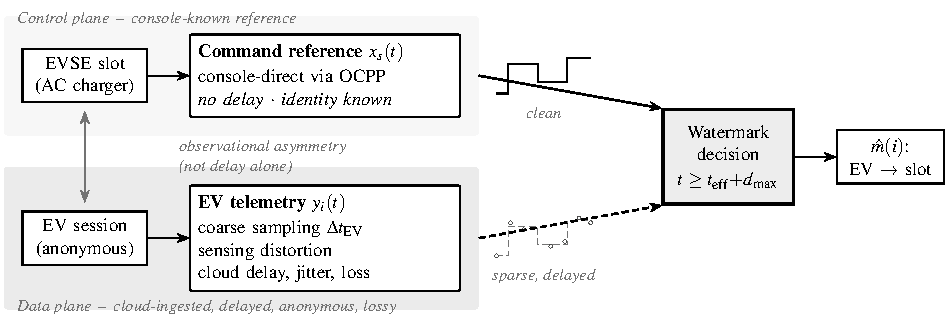
\includegraphics[width=\textwidth]{figure1_two_plane_observability.pdf}}
        \caption{\revised{Two-plane observability in the proposed EV--charger matching problem. The control plane (EVSE current reference $x_s(t)$, whose slot label is known) is read directly from the OCPP console without uplink delay, whereas the data plane (EV-side telemetry $y_i(t)$, session-identified but carrying no EVSE-slot label) reaches the backend after sensing distortion, cloud-ingestion delay, jitter, and loss. Finalization fires at $t \geq t_{\text{eff}} + d_{\max}$ (Section~III-B); {\unboldmath$\Delta t_{\text{EV}}$} is the EV sampling period.}}
        \label{fig01}
    \end{figure*}
    \section{RELATED WORK}

    \revised{Smart charging and V2G operation~\cite{b2,b3,b5} presuppose that the charging backend knows which EV is connected to each EVSE slot.}
    Prior work related to this requirement falls into three groups: EV identification from charging behavior, matching and assignment within EV charging systems, and online evidence integration under delayed telemetry.
    However, these studies do not directly resolve the present setting, where the EV--EVSE association must be recovered online from delayed, \revised{slot-unlabeled}, and imperfect EV-side telemetry on legacy IEC~61851 AC infrastructure.

    \subsection{EV Identification From Charging Behavior}
    Non-intrusive load monitoring~\cite{bhart} established that an electrical load carries identifying information.
    \revised{EV charging in particular has a characteristic load behavior at the distribution level~\cite{b9}, and its session data support brand-and-model classification~\cite{b10}, per-vehicle fingerprinting~\cite{b11}, and session-duration-class classification~\cite{b12}.}
    Recent work pushes this further toward earlier and finer-grained EV-instance recognition from early-charging voltage patterns~\cite{bmarchiori25}.
    \revised{Adjacent work makes an EV's charging power track a reference through the standard AC interface~\cite{bferretti24}, or estimates battery state: state of charge from a cell model~\cite{b20} or from the active power drawn at the charging socket~\cite{b21}, and second-life state of health from first-life data and on-board voltage measurements alone~\cite{bjameel24}.}
    \revised{Charging behavior thus carries load-, session-, vehicle-, and battery-level information; the identification studies answer \emph{what kind of vehicle} or \emph{which previously enrolled vehicle} is charging, but none of these works answers the operational pair question of \emph{which of several concurrently active EVs is on which EVSE slot} from delayed, slot-unlabeled cloud telemetry alone.}

    \subsection{Matching and Assignment in EV Charging Systems}
    EV-charging-specific matching has been studied for several operational questions, including stable matching for subscription-based service models~\cite{bkhanda} and capacity-aware top trading cycles for post-choice reassignment in shared cyber-physical charging environments~\cite{breactttc}.
    These works presume declared user preferences, known vehicle identities, and timely coordination channels, and frame the operational question as how to \emph{allocate} or \emph{reassign} EVs across stations.
    The present setting is not an allocation problem in that sense: the EV is already physically connected, and the task is to \emph{recover} the missing physical-to-logical pair link from \revised{slot-unlabeled}, delayed, waveform-only evidence.

    \subsection{Sequential Association and Delayed Telemetry}
    The methodological tools for committing one-to-one decisions under partial and uncertain evidence are well established.
    Online bipartite matching~\cite{b17,b18}, \revised{with extensions in which a match may be deferred at a delay cost~\cite{bemek16}}, supplies the formal assignment basis.
    Recursive Bayesian filtering~\cite{b19,bsarkka} motivates the posterior-updating \revised{rule of the Posterior matcher}, applied here to \revised{slot-unlabeled}, asymmetric, delay-bounded EV-current telemetry rather than to spatially resolved, time-synchronous measurements.

    A parallel telemetry-side literature characterizes the \revised{acquisition and} delay envelope within which an online matcher must decide.
    \revised{Wireless energy-monitoring prototypes relay voltage and current samples from sensor nodes to a nearby host at tens of hertz over a short radio link~\cite{bsabry17}, whereas cloud-ingested EV-side telemetry arrives coarsely sampled, after a delay that is itself uncertain.}
    The Open Charge Point Protocol (OCPP)~\cite{b22}, the underlying WebSocket~\cite{b23} over Transmission Control Protocol (TCP)~\cite{b24} transport, and broadband-latency baselines~\cite{b25} motivate bounded low-second-scale ingestion assumptions.
    Formal watermark semantics from event-time stream processing~\cite{b26} then supply the rule by which delayed evidence is judged mature enough for irrevocable finalization.
    \revised{This strand characterizes acquisition rates, transport delay and loss, and data maturity in isolation}, but does not address how to integrate the resulting delayed evidence into a \revised{one-to-one EV--EVSE assignment}.

    Taken together, the three strands offer vehicle-level information, \revised{allocation mechanisms for EVs whose identities are known, and tools for one-to-one decisions under delayed, uncertain evidence}, but none combines them for pair-level EV--EVSE identification in the present setting.
    \revised{The present work addresses this gap with a watermark-based online runtime inside which waveform-based matchers are compared against a timing-only baseline.}

    \section{SYSTEM MODEL AND PROBLEM FORMULATION}

    Building on the measurement-based current-generation model used in prior MCCT work~\cite{b14}, this section defines the additional online decision layer required when EV-side observations are not available as a complete batch but arrive through delayed \revised{slot-unlabeled} telemetry.

    \subsection{Operational Objective and Two-Plane Observability}
    Let $i \in E$ denote an EV session and $s \in S$ denote an EVSE slot, where $E$ and $S$ are the session and slot sets.
    The operational objective is to emit an online finalized mapping $\hat{m}(i) \in S$ that matches the true EVSE slot of session $i$, with one-to-one consistency enforced among simultaneously finalized matches.
    Each EVSE slot is physically exclusive: at any time $t$, slot $s$ hosts at most one session, so for any two sessions $i \neq j$ admitted to the same slot ($m(i) = m(j) = s$, where $m$ denotes the true admission mapping\revised{, i.e., $m(i)=s$ means that session $i$ is connected to slot $s$}) the active intervals $[t_{\text{arr},i}, t_{\text{end},i}]$ (from arrival $t_{\text{arr},i}$ to session end $t_{\text{end},i}$) are disjoint.
    An arriving EV is admitted to a slot that is free at $t_{\text{arr},i}$; admission scheduling is therefore not a degree of freedom of the matcher.

    The system model contains two observation planes (Fig.~\ref{fig01}) that explicitly separate the EVSE-side reference (control plane, console-direct) from the EV-side telemetry (data plane, cloud-ingested).
    This separation is conceptually consistent with the information-and-communication-technology (ICT)--energy-equipment decomposition reference model of Imanaka~\textit{et al.}~\cite{bimanaka23} and with the broader edge-cloud architectural perspective of Satyanarayanan~\cite{bsatya}.
    The control plane provides the console-known EVSE reference stream $x_s(t)$ for each slot $s$.
    The reference is generated from the MCCT command pattern through the data-driven model in Section~V-A.
    The charger is remotely commanded via OCPP, and the charger-cloud log is directly accessible at the control console~\cite{b14}.
    This stream is therefore treated as known without uplink delay.
    The data plane provides \revised{a slot-unlabeled} EV observation stream $y_i(t)$ for each EV session $i$.
    The stream is observed only after asynchronous ingestion with the impairments described in Section~V-A.
    The two-plane asymmetry---not delay alone---is the defining feature of this problem.
    \revised{The same asymmetry arises in other cyber-physical systems where commands are known on one plane and responses arrive delayed and unlabeled on another, such as attributing consumption to tenants behind a shared meter or linking controller setpoints to cloud-ingested sensor streams; the formulation below therefore applies beyond EV charging, which is the case calibrated and evaluated here.}

    \subsection{Window--Watermark Online Decisioning}
    The MCCT observation window has duration
    \begin{equation}\label{eq:e1}
        W = \tau \cdot N_{\text{steps}},
    \end{equation}
    where $\tau = 60$\,\text{sec} and $N_{\text{steps}} = 6$, yielding $W = 360$\,\text{sec}.
    This window length follows the MCCT observation convention of prior work~\cite{b13},~\cite{b14}, keeping the matching task directly comparable.
    \revised{The backend does not observe the physical arrival $t_{\text{arr},i}$; it observes the EV-side start estimate $\hat{t}_{\text{start},i}$ (the first EV sample at or above 1\,A, with jitter; Section~V-A) and the end timestamp $\hat{t}_{\text{end},i}$ reported by the EV-side stream itself.
    The nominal decision-window end is $t_{\text{win},i} = \hat{t}_{\text{start},i} + W$.}
    The runtime does not, however, finalize exactly at $t_{\text{win},i}$ because EV-side telemetry may still be in transit.
    Instead, it waits until a watermark condition is satisfied: in event-time stream processing, a watermark marks the time by which all records with earlier event times are assumed to have arrived~\cite{b26}; here it bounds when the delayed EV-side prefix of session $i$ is complete enough for an irrevocable pairing decision.
    Let $d_{\max}$ denote the watermark delay bound.
    \revised{In this study $d_{\max}$ is a fixed design constant set at the commercial OCPP message-timeout default (Section~V-A); an adaptive bound is discussed in Section~VII-C.}
    The watermark-ready time is
    \begin{equation}\label{eq:e2}
        t_{\text{wm},i} = t_{\text{eff},i} + d_{\max},
    \end{equation}
    where the effective end time is defined as
    \begin{equation}\label{eq:e3}
        \revised{t_{\text{eff},i} = \min\!\left(\hat{t}_{\text{start},i} + W,\; \hat{t}_{\text{end},i}\right).}
    \end{equation}
    The $\min$ clamp advances the watermark to the actual end when a session closes before the nominal window, preventing the watermark from overshooting into a future that will never be observed.
    An EV session is mature when $t \geq t_{\text{wm},i}$, which bounds waiting: deciding too early yields a too-short EV prefix, waiting too long degrades online usefulness.

    \subsection{Candidate Gating, Assignment, and Finalization Semantics}
    The candidate slot set for EV session $i$ is restricted to slots active near the effective end.
    Let $\Delta$ denote the candidate time margin.
    Then
    \begin{equation}\label{eq:e4}
        \revised{C_i = \{ s \in S \mid s \text{ active in } [t_{\text{eff},i} - \Delta,\, \min(t_{\text{eff},i} + \Delta,\, t_{\text{final},i})] \},}
    \end{equation}
    \revised{where $t_{\text{final},i} \geq t_{\text{wm},i}$ is the evaluation tick at which session $i$ is decided.}
    Candidate gating reduces computational burden and narrows matching to operationally plausible slots; the upper bound is clamped \revised{at that decision tick, so that} gating never uses slot activity observed after the decision, preserving online causality.
    If $C_i$ is empty, the runtime falls back to the full EVSE-slot set $S$ and records the fallback invocation (which remains zero in the base-load regime).
    \revised{The gate can exclude the true slot only if its inputs are wrong: an EV-side start or end estimate displaced by more than $\Delta$ (e.g., through clock skew between the planes or a lost end record), or a missing slot-activity record.}
    When several mature EV sessions are processed together, the runtime constructs a cost matrix $\mathbf{C} = [c_{i,s}]$ (distinct from the candidate set $C_i$) and solves
    \begin{equation}\label{eq:e5}
        \min_\pi \sum_i c_{i,\pi(i)} \quad \text{s.t.} \quad \pi(i) \in C_i,\; \pi(i) \neq \pi(j)\;\text{for}\;i \neq j.
    \end{equation}
    The compared algorithms differ in how $c_{i,s}$ is computed, and the finalized mapping emitted by the runtime satisfies $\hat{m}(i) = \pi(i)$. \revised{The one-to-one constraint applies within one batch: a slot finalized in an earlier batch is not reserved, so two sessions can be finalized to the same slot, in which case at least one of them is misidentified and counted as an error (Section~VII-E).}
    An EV session is \textit{admitted} if it can be scheduled onto an available EVSE slot, and \textit{blocked} if no capacity is available.
    A session is \textit{finalized} when the runtime emits an EV--charger match.
    Finalization occurs through ordinary watermark-based maturity or\revised{, when a session ends before its watermark or the scenario ends, through the fallback path}.
    The watermark maturity rule, candidate gating in Eq.~\eqref{eq:e4}, and per-batch one-to-one finalization are shared by all four matchers studied in Section~IV.
    Matcher-specific extensions are limited to the Posterior matcher, which builds a per-session posterior through two update stages before assignment costs are computed.

    \subsection{Evaluation Metrics}
    Three primary metrics are reported: \revised{admitted-session accuracy} $\tfrac{N_{\text{correct}}}{N_{\text{admitted}}}$, requested-session accuracy $\tfrac{N_{\text{correct}}}{N_{\text{requested}}}$, and 90th-percentile decision latency $\text{Quantile}_{0.9}(\{t_{\text{final},i} - t_{\text{arr},i}\})$, where $N_{\text{requested}}$ counts all arriving sessions (admitted plus blocked) and $t_{\text{final},i}$ is the finalization time; the first two coincide at low load and diverge only under saturation, where requested-session accuracy becomes the operationally meaningful measure \revised{(exercised in Section~VI-A)}, and candidate-set composition (average count, ground-truth retention, fallback invocations) is recorded as auxiliary diagnostic.

    \begin{figure*}[!t]
        \centerline{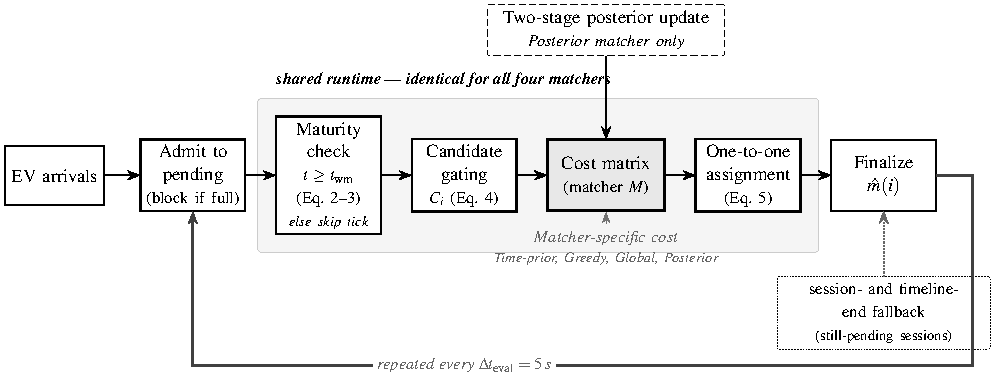
\includegraphics[width=\textwidth]{figure2_event_driven_runtime.pdf}}
        \caption{Shared event-driven runtime used by all compared matchers. The entire loop---arrivals, maturity, candidate gating, cost-matrix construction, assignment, and finalization---re-runs at every evaluation tick ({\unboldmath$\Delta t_{\mathrm{eval}} = 5$\,\text{sec}}). All four matchers use identical watermark maturity, candidate gating, batch construction, and per-batch one-to-one finalization timing; \revised{they differ in cost-matrix construction and, for the Greedy matcher, in the one-to-one solver (greedy rather than Hungarian; TABLE~\ref{table2})}. The Posterior matcher additionally applies a two-stage posterior update before constructing the cost matrix.}
        \label{fig02}
    \end{figure*}
    \section{\revised{RUNTIME AND COMPARED MATCHERS}}

    This section presents the four matchers compared in this study, all of which operate inside the shared event-driven runtime introduced in Section~III.

    \subsection{Event-Driven Runtime}
    The runtime is explicitly event-driven with evaluation interval $\Delta t_{\text{eval}} = 5$\,\text{sec}.
    At each evaluation tick the runtime updates the pending session set, checks maturity via $t_{\text{wm}} = t_{\text{eff}} + d_{\max}$ with $t_{\text{eff}}$ clamped per Eq.~\eqref{eq:e3}, constructs candidate slot sets via Eq.~\eqref{eq:e4} with margin $\Delta$, evaluates pairwise compatibility on the watermark-visible prefix, builds a cost matrix over the matured batch, and solves one-to-one assignment.
    Fig.~\ref{fig02} shows this shared loop; its shared band marks the components common to all four matchers\revised{,} isolating the cost-matrix block as the \revised{main} divergence point among Time-prior, Greedy, Global, and Posterior.
    With maturity, gating, and timing held identical, the accuracy differences reported in Section~VI are attributable to cost construction\revised{, belief updating, and, for the Greedy matcher, the assignment solver}.

    \subsection{\revised{The Four Compared Matchers}}
    The Time-prior, Greedy, and Global matchers are single-shot decisions that differ \revised{mainly} in cost-matrix construction.
    The Posterior matcher additionally uses a two-stage posterior update before the shared assignment step (TABLE~\ref{table2}).

    \begin{table}[htbp]
        \caption{Matcher design summary. \revised{Only the Posterior matcher uses an explicit two-stage posterior update, separating it structurally from the three single-shot matchers.}}
        \label{table2}
        \centering
        \setlength{\tabcolsep}{3pt}
        \scriptsize
        \begin{tabular}{@{}l p{2.1cm} p{1.5cm} p{1.3cm}@{}}
            \toprule
            \textbf{Matcher} & \textbf{Primary evidence} & \textbf{Assignment} & \textbf{Posterior update} \\
            \midrule
            Time-prior & Timing only & Hungarian & None \\
            Greedy & DTW + step-sig. & Greedy 1:1 & None \\
            Global & Correlation + DTW & Hungarian & None \\
            Posterior & Bayesian posterior & Hungarian & Two-stage \\
            \bottomrule
        \end{tabular}
    \end{table}

    \textbf{Time-prior baseline.}
    The time-prior baseline is a timing-only reference that ignores waveform shape entirely; compatibility is the temporal-proximity cost
    \begin{equation}\label{eq:a0}
        c^{(A0)}_{i,s} = D_{\text{end}}(t_{\text{eff},i}, s) + 0.10\,D_{\text{start}}(\revised{\hat{t}_{\text{start},i}}, s),
    \end{equation}
    where $D_{\text{end}}$ is the \revised{distance from $t_{\text{eff},i}$ to the nearest active interval of slot~$s$ (zero when $t_{\text{eff},i}$ lies inside one)} and $D_{\text{start}}$ is the minimum distance from the EV start-estimate to any slot-$s$ active start, after which Hungarian assignment is applied.
    It is a quantitative anchor rather than a competitive method; its gap to the other three matchers isolates the value of waveform evidence.

    \textbf{Greedy waveform matcher.}
    The greedy waveform matcher evaluates a pairwise cost from the EV prefix and the EVSE-slot prefix:
    \begin{equation}\label{eq:e6}
        c^{(A1)}_{i,s} = \lambda_{\text{dtw}}\,d^{\text{dtw}}_{i,s} + \lambda_{\text{step}}\,d^{\text{step}}_{i,s} + \lambda_{\text{mean}}\,d^{\text{mean}}_{i,s},
    \end{equation}
    where $d^{\text{dtw}}$ is a band-constrained DTW discrepancy~\cite{b16} \revised{(Sakoe--Chiba band of $\pm 15$\,\text{sec}, i.e., three 5\,\text{sec} samples)} computed on z-normalized prefixes and divided by the prefix length, $d^{\text{mean}}$ is the mean-gap term, and $d^{\text{step}}$ is the step-signature discrepancy computed on per-step medians as
    \begin{equation}\label{eq:e7}
        d^{\text{step}}_{i,s} = \text{mean}|e_{\text{sig}} - s_{\text{sig}}|,
    \end{equation}
    in which $e_{\text{sig}}$ and $s_{\text{sig}}$ are step medians (in amperes) over each $\tau$-second sub-window, so $d^{\text{step}}$ is in amperes and penalizes local mismatch on the same temporal grid as the MCCT step pattern.
    The default constants are $\lambda_{\text{dtw}} = 1.0$, $\lambda_{\text{step}} = 0.40$, $\lambda_{\text{mean}} = 0.0$; calibration on the calibration slice (Section~V-C) showed $d^{\text{mean}}$ to be subsumed by the DTW term at this sampling rate, so the Greedy matcher effectively operates on DTW plus the step-signature cost.
    \revised{The sessions of a matured batch are taken in decreasing order of the margin between their two lowest candidate costs, and each is assigned its lowest-cost slot not yet taken (greedy one-to-one selection)}, providing a lightweight waveform baseline.

    \textbf{Global waveform assignment.}
    \revised{This matcher carries the prior static correlation--DTW cost of~\cite{b14} unchanged into the runtime; it is labeled Global in the tables and figures and called the prior static cost in the text.}
    The global waveform assignment computes a combined waveform score from normalized correlation $\rho^{\text{norm}}$ and normalized DTW $\delta^{\text{norm}}$:
    \begin{equation}\label{eq:e8}
        \text{eval}_{i,s} = \rho^{\text{norm}}_{i,s} \cdot \delta^{\text{norm}}_{i,s},
    \end{equation}
    \begin{equation}\label{eq:e9}
        c^{(A2)}_{i,s} = 1 - \text{eval}_{i,s}.
    \end{equation}
    Correlation is mapped from $[-1, 1]$ to $[0, 1]$ via
    \begin{equation}\label{eq:rhonorm}
        \rho^{\text{norm}} = \frac{\rho + 1}{2}.
    \end{equation}
    The DTW distance \revised{(on the raw currents, without a band)} is first normalized by the alignment-path length to remove sequence-length bias.
    It is then min--max scaled across the finite candidate pairs of the matured batch (when all values coincide, $\delta^{\text{norm}} = 1$ for every pair), giving the normalized similarity
    \begin{equation}\label{eq:deltanorm}
        \delta^{\text{norm}} = 1 - \text{MinMax}(\text{DTW}_{\text{path}}).
    \end{equation}
    The resulting dense cost matrix is passed to Hungarian assignment~\cite{b15}.

    \textbf{Two-stage posterior matcher.}
    The two-stage posterior matcher is a runtime-integrated Bayesian matcher designed for \revised{slot-unlabeled}, delayed EV telemetry \revised{with per-batch one-to-one assignment}.
    At each watermark decision for a mature batch, it performs two posterior-update stages over each candidate set.
    Following recursive Bayesian filtering~\cite{b19},~\cite{bsarkka}, update stage $k$ combines a timing prior $P_t(s|i)$, a current-based likelihood $P_c(s|i)$, and the previous within-decision posterior $P_{k-1}(s|i)$ through
    \begin{equation}\label{eq:e10}
        P_k(s|i) \propto P_{k-1}(s|i)^{\gamma_{\text{prev}}} \cdot P_t(s|i)^{\gamma_t} \cdot P_c(s|i),
    \end{equation}
    where $\gamma_{\text{prev}}$ and $\gamma_t$ weight the within-decision carry-over belief relative to the current stage's waveform evidence.
    The current-based likelihood is a scale-normalized softmax over the candidate set,
    \begin{equation}\label{eq:pc}
        P_c(s|i) = \frac{\exp\!\big(-\beta_{\text{curr}}\,\frac{c_{i,s}-c_i^{\min}}{\sigma_i}\big)}{\sum_{s'\in C_i}\exp\!\big(-\beta_{\text{curr}}\,\frac{c_{i,s'}-c_i^{\min}}{\sigma_i}\big)},
    \end{equation}
    where $c_{i,s}$ is the refined DTW and step-signature waveform cost (cf.\ Eq.~\eqref{eq:e6}--\eqref{eq:e7}) on the watermark-visible prefix, $c_i^{\min}=\min_{s\in C_i}c_{i,s}$, and $\sigma_i$ is the median absolute deviation of $\{c_{i,s}\}_{s\in C_i}$ (if it falls below $10^{-6}$, the standard deviation is used instead, then the value range, then unity); the two update stages evaluate $c_{i,s}$ on the first $60\%$ and on the full matured prefix, respectively (TABLE~\ref{table:hyper}).
    \revised{The number of stages was chosen empirically on the calibration slice: the 60\,\% prefix already separated most candidates and the full prefix resolved the rest, whereas a third stage would re-score largely the same samples at the cost of one more waveform evaluation per candidate.
    Because both stages score the same series, Eq.~\eqref{eq:e10} acts as a tempered evidence update rather than a product of independent likelihoods.}
    The time prior $P_t(s|i)$ \revised{decays with the distance $\Delta\tau_{i,s}$ from $t_{\text{eff},i}$ to the nearest active interval of the candidate slot (zero when the slot is active at $t_{\text{eff},i}$)}: writing $q^{75}_i$ for the $75$th percentile of $\{\Delta\tau_{i,s}\}_{s\in C_i}$ (floored at 1\,\text{sec}), the shaped prior is
    \begin{equation}\label{eq:shaped}
        P_t^{\text{shaped}}(s|i)\propto\exp\!\left(-\alpha_{\text{time}}\,\frac{\Delta\tau_{i,s}}{q^{75}_i}\right),
    \end{equation}
    blended with a uniform prior over $C_i$ as
    \begin{equation}\label{eq:ptblend}
        P_t = \eta_{\text{mix}}\,P_t^{\text{shaped}} + (1-\eta_{\text{mix}})\,P_t^{\text{uniform}},
    \end{equation}
    to prevent early posterior collapse on sparse evidence.
    At the first update stage ($k = 1$), the carry-over factor in Eq.~\eqref{eq:e10} is initialized as a uniform prior over $C_i$.
    Eq.~\eqref{eq:e10} is renormalized over $s \in C_i$ after every update.
    The $\alpha$, $\beta$, $\gamma$, \revised{$\eta$,} and $\lambda$ hyperparameter family is listed in TABLE~\ref{table:hyper} together with the calibration basis.
    Assignment costs blend the posterior log-cost with the last stage's current-likelihood log-cost,
    \begin{equation}\label{eq:e11}
        c^{(A3)}_{i,s} = (1 - \lambda_{\text{blend}})\,(-\log P_k(s|i)) + \lambda_{\text{blend}}\,(-\log P_c^{\text{last}}(s|i)),
    \end{equation}
    with $\lambda_{\text{blend}} = 0.15$ (TABLE~\ref{table:hyper}); $P_k$ is renormalized over $s \in C_i$ after each update.
    The Posterior matcher is the only method that constructs assignment costs from an explicit posterior state.

    \begin{table}[htbp]
    \caption{Hyperparameter values and calibration basis. All values are fixed on the calibration slice and frozen before any evaluation run.}
    \label{table:hyper}
    \centering
    \scriptsize
    \setlength{\tabcolsep}{3pt}
    \begin{tabular}{@{}l l p{4.2cm}@{}}
        \toprule
        \textbf{Symbol} & \textbf{Value} & \textbf{Calibration basis} \\
        \midrule
        $\lambda_{\text{dtw}}$ & $1.0$ & Unit-normalized weight on the DTW term \\
        $\lambda_{\text{step}}$ & $0.40$ & Selected on the calibration slice (Section~V-C) \\
        $\lambda_{\text{mean}}$ & $0.0$ & Mean-gap subsumed by DTW at this sampling rate \\
        $\gamma_{\text{prev}}$ & $0.60$ & Within-decision carry-over exponent (both stages) \\
        $\gamma_t^{(1)}$, $\gamma_t^{(2)}$ & $1.00$ and $0.20$ & Time-prior exponent at Stage~1 and Stage~2 \\
        $\alpha_{\text{time}}$ & $1.0$ & Timing-prior decay rate \\
        $\eta_{\text{mix}}$ & $0.35$ & Weight on shaped time-prior in $\eta_{\text{mix}}\,\text{shaped}+(1{-}\eta_{\text{mix}})\,\text{uniform}$ \\
        $\beta_{\text{curr}}$ & $1.0$ & Unit scale on current-based likelihood \\
        $\lambda_{\text{blend}}$ & $0.15$ & Small blend weight in $c^{(A3)}$ (Eq.~\eqref{eq:e11}); kept low so the posterior term dominates the blended cost \\
        \revised{Stage prefixes} & \revised{$60\,\%$ / $100\,\%$} & \leavevmode\revised{Share of the matured prefix scored at Stage~1 / Stage~2} \\
        \revised{DTW band} & \revised{$\pm 15$\,\text{sec}} & \leavevmode\revised{Sakoe--Chiba band of $d^{\text{dtw}}$ (three 5\,\text{sec} samples)} \\
        \bottomrule
    \end{tabular}
    \end{table}

    \subsection{Hyperparameter Selection}
    The $\alpha$, $\beta$, $\gamma$, \revised{$\eta$,} and $\lambda$ weights are fixed on a small held-out calibration slice and frozen before any evaluation run.
    The explicit calibration-versus-evaluation partition is given in Section~V-C, so the reported \revised{comparison} is independent of the tuning signal.
    Numerical values of all hyperparameters are listed in TABLE~\ref{table:hyper} together with the calibration basis for each value.
    \revised{Section~VI-B reports the sensitivity to $\gamma_{\text{prev}}$, $\eta_{\text{mix}}$, and $\beta_{\text{curr}}$.}
    \section{EXPERIMENTAL SETUP}

    \subsection{Simulator and Signal Model}

    The simulation environment rests on three layers with decreasing empirical grounding: a measurement-based current-generation model that produces the \revised{charging current of every session, observed on both planes} (Layer~1), an event-driven session-level runtime that schedules asynchronous EV arrivals and departures (Layer~2), and a cloud-ingestion model that determines how EV-side observations reach the backend (Layer~3).
    Although the present study is simulation-based, its signal foundation is measurement-derived: Layer~1 reuses the data-driven current-generation model that Nomura~\textit{et al.}~\cite{b14} fitted to real Wallbox Pulsar Plus and Tesla Model~3 current measurements \revised{(an input--output response model identified from measured data, in the manner of data-driven system identification~\cite{bbakirci23})}, so the simulated waveforms retain measured response features from that Wallbox--Tesla equipment pair rather than idealized step shapes.

    \textbf{Layer~1: Measurement-based current-generation model.}
    The charger-side command sequence follows a fixed six-step MCCT-style structure with $\tau = 60$\,\text{sec} (yielding an observation window of $W = 360$\,\text{sec}), and the EVSE-side reference is generated through the data-driven response model of Nomura~\textit{et al.}~\cite{b14}, fitted from EV and EVSE current measurements collected on a Wallbox Pulsar Plus AC charger and a Tesla Model~3 RWD Standard Range Plus under the original Baba--Imanaka equipment setup~\cite{b13}; as reported by Nomura~\textit{et al.}~\cite{b14}, these measurements were obtained from the YourStand AC charging-service deployment.
    The model captures three behaviors---delayed change onset, target-current offset, and asymmetric ramp---broadly consistent with real-world AC-charging current behavior reported in independent measurement-based studies~\cite{bferretti24}.
    The command-to-current response lag used for waveform generation is modeled as 15\,\text{sec} for the first nonzero charging step and 5\,\text{sec} for subsequent setpoint changes.
    The 15\,\text{sec} value is treated as a waveform-generation assumption informed by the EV charging full-activation-time (FAT) ranges reported by Imanaka and Baba~\cite{bimanaka25}.
    These values do not represent backend telemetry-arrival delay, which is modeled separately in the cloud-ingestion layer.
    The remaining fitted parameters are
    \begin{equation}\label{eq:e14}
        I_{\text{offset}} = 0.0221\,u + 0.2831,
    \end{equation}
    \begin{equation}\label{eq:e15}
        \Delta I_{\text{rise}} = 0.0327\,\Delta u + 0.3787,
    \end{equation}
    where $u$ is the commanded current setpoint (A), $\Delta u$ is the setpoint change between consecutive steps (A), $I_{\text{offset}}$ is the steady-state command-to-current offset (A), and $\Delta I_{\text{rise}}$ is the current rise rate (A/s).
    For falling transitions, the current decreases at a maximum rate of 4\,A per second, and the resulting EVSE current is rounded to 0.1\,A; this prevents the matching problem from being defined over an unrealistically ideal waveform.
    The EVSE reference \revised{sampling period} is five seconds.
    \revised{To test the dependence on this single fitted response, Section~VI-B also draws, per session, the first-step lag from $U(2, 30)$\,\text{sec} and the rise rate from $U(1, 10)$\,A/s (fall rate capped at $\min(4, r)$\,A/s); the drawn dynamics appear on both planes, and the matchers never evaluate Eqs.~\eqref{eq:e14}--\eqref{eq:e15}.
    Every non-zero setpoint lies in 6--30\,A, inside the operator's normal range, and the first step sets 0\,A; the pattern is re-issued every $W$, and each session is decided on its first window.}

    \textbf{Layer~2: Online event-driven session model.}
    The online contribution of this study begins at the runtime layer: sessions are no longer assumed to be simultaneous or complete at the time of matching.
    The simulator configures a single site with fifty EVSE slots (charging ports) and a twelve-hour scenario horizon; the fifty-slot capacity provides a multi-port site setting for evaluating online matching under moderate candidate ambiguity, and together with sessions of ten to sixty minutes it keeps the evaluated EV-session count (up to 500 sessions) below saturation in the \revised{base-load} envelope.
    Arrival times are sampled independently and uniformly over the first eleven hours of the horizon and then sorted. Session durations are sampled uniformly from ten to sixty minutes, inclusive. Each arriving session is admitted to a slot chosen uniformly at random among the slots free at its arrival time, using the seeded scenario random-number generator, under the slot-exclusivity constraint of Section~III-A; if no slot is free, the session is blocked.
    Each six-step command pattern starts at $0$\,A and is followed by five distinct setpoints drawn \revised{uniformly at random} from $\{6,\dots,30\}$\,A\revised{; a seeded pool of fifty unique patterns is kept per scenario, and each arriving session receives the free pattern farthest from those of the active sessions by a mainly z-normalized shape distance.
    The farthest-point generator cannot attain a separation floor for fifty patterns and falls back to a random draw, so the pool is effectively random: the minimum pairwise $\ell_1$ setpoint distance is 4--13\,A per repeat and the mean pairwise distance is 42\,A; Section~VI-B narrows the setpoint band.}

    \textbf{Layer~3: Cloud-ingestion and telemetry imperfection.}
    The EV-side signal is formed by applying sensing distortion to the EVSE-side current: each session is assigned an uncalibrated EV--EVSE waveform-coordinate offset (a fixed 5\,\text{sec} component plus a uniform draw from 0 to 20\,\text{sec}; distinct from acquisition and cloud-ingestion delay), start-estimate jitter \revised{(uniform over $\pm 20$\,\text{sec}; the estimate is kept within $[t_{\text{arr},i} - \Delta t_{\text{EV}},\, t_{\text{arr},i} + W/2]$)}, multiplicative gain variation (std~0.03\revised{, clipped to $[0.8, 1.2]$}), and additive bias (std~0.35\,A), and each sample carries additive noise (std~0.20\,A).
    \revised{Each EV-side sample reads the slot current at its offset time and is rounded up to the next ampere.
    Ingestion delay and measurement loss are drawn once per EV-side measurement (mean delay 2.0\,\text{sec}, jitter 1.0\,\text{sec}, loss probability 0.005; TABLE~\ref{table3}); for a lost measurement the decision grid holds the last received value.
    These three values} are engineering assumptions that fix a low-second-scale ingestion envelope, not field measurements of a specific EV-cloud service. \revised{Section~VI-B sweeps loss, delay, and sensing distortion well beyond them.} The cited transport and broadband references~\cite{b23},~\cite{b24},~\cite{b25} motivate only the order of magnitude; because network round-trip is sub-second, the 2.0\,\text{sec} mean represents application-level ingestion rather than transport delay. The 10.0\,\text{sec} ingestion-delay cap follows the commercial OCPP MessageTimeout default~\cite{bzaptec},~\cite{b22} and is distinct from the decision-side watermark bound $d_{\max}$ of Eq.~\eqref{eq:e2}.
    The numerical results in Section~VI should be read as statements about this evaluation envelope and the \revised{comparison of} the four matchers, not as absolute field predictions.

    \begin{table}[htbp]
        \caption{Cloud-ingestion defaults used to define the evaluation envelope; references provide operational defaults or order-of-magnitude proxies, not field calibration for a specific EV-cloud service.}
        \label{table3}
        \centering
        \small
        \setlength{\tabcolsep}{3pt}
        \begin{tabular}{@{}p{2.6cm} p{1.2cm} p{3.4cm}@{}}
            \toprule
            \textbf{Parameter} & \textbf{Default} & \textbf{Basis or proxy} \\
            \midrule
            Mean ingestion delay & 2.0\,\text{sec} & WebSocket and TCP~\cite{b23},~\cite{b24} \\
            Delay jitter (std) & 1.0\,\text{sec} & TCP retransmission~\cite{b24} \\
            Ingestion-delay cap & 10.0\,\text{sec} & OCPP MessageTimeout~\cite{bzaptec} \\
            \leavevmode\revised{Measurement-loss probability (per EV-side measurement)} & 0.005 & \leavevmode\revised{FCC broadband packet loss, sub-1\%, as an order-of-magnitude proxy}~\cite{b25} \\
            EVSE-side delay and loss & None & Console-direct \\
            EV sampling period $\Delta t_{\text{EV}}$ & 30\,\text{sec} & OCPP MeterValue interval~\cite{babb} \\
            \bottomrule
        \end{tabular}
    \end{table}

    \subsection{Evaluation Design}
    The main base-load comparison uses EV-session counts of 100, 300, and 500 with 20 repeated simulations per operating point.
    Additional experiments vary \revised{EV sampling period} (5, 15, 30\,\text{sec}), watermark delay bound (5, 10, 15\,\text{sec}), and candidate margin (60, 120, 180\,\text{sec}).
    \revised{On the same seeds and protocol, Section~VI adds impairment, heterogeneity, codebook, and hyperparameter sweeps, two saturation points, and diagnostic runs.}
    Error bars denote 95\,\% confidence intervals from the evaluation repeats at each operating point (20 repeats at $EV \in \{100,500\}$ and the 15 held-out repeats at $EV=300$)\revised{, with Student's $t$ quantiles for paired differences and where a caption states it, and} under a normal approximation \revised{otherwise}.
    The default experimental preset is summarized in TABLE~\ref{table5}.
    \begin{table}[!t]
        \caption{Operating-point grid for base-load and sensitivity evaluation; results are drawn from the held-out remainder. Representative point: {\unboldmath $(EV, \Delta, d_{\max}, \Delta t_{\mathrm{EV}}) = (500, 120~\mathrm{s}, 10~\mathrm{s}, 30~\mathrm{s})$}.}
        \label{table5}
        \centering
        \begin{tabular}{ll}
            \toprule
            \textbf{Item} & \textbf{Value} \\
            \midrule
            EV-session-count sweep & 100, 300, 500 \\
            Repeats & 20 \\
            Pattern mode & current \\
            Pattern assignment mode & dynamic session \\
            Pattern unique count & 50 \\
            Command step count & 6 \\
            $\tau$ values & 60\,\text{sec} \\
            \revised{EV sampling period sweep} & 5\,\text{sec}, 15\,\text{sec}, 30\,\text{sec} \\
            Watermark delay bound $d_{\max}$ sweep & 5\,\text{sec}, 10\,\text{sec}, 15\,\text{sec} \\
            Candidate margin $\Delta$ sweep & 60\,\text{sec}, 120\,\text{sec}, 180\,\text{sec} \\
            Error bars & 95\,\% confidence interval \\
            \bottomrule
        \end{tabular}
    \end{table}

    \begin{table}[!t]
        \caption{Calibration and evaluation slices are drawn from disjoint repeats, so that reported accuracy, latency, and ablation results are independent of the tuning signal.}
        \label{table:calib_eval}
        \centering
        \begin{tabular}{p{2.0cm} p{2.5cm} p{2.7cm}}
            \toprule
            \textbf{Purpose} & \textbf{Data slice} & \textbf{Used for} \\
            \midrule
            Hyperparameter tuning (calibration) & $EV~=~300$, repeats 1--5 & $\alpha$, $\beta$, $\gamma$, \revised{$\eta$,} $\lambda$ \\
            Evaluation (main) & $EV \in \{100, 500\}$, repeats 1--20; $EV~=~300$, repeats 6--20 & Fig.~\ref{fig05}, TABLE~\ref{table6}, Section~VI-A \\
            Sensitivity & Same repeats as main + parameter sweeps ($\Delta t_{\text{EV}}$, $d_{\max}$, $\Delta$\revised{; impairments, heterogeneity, setpoint band, hyperparameters, saturation, static limit}) & Section~VI-\revised{A, VI-}B \\
            Ablation & Same repeats as main \revised{(+ two-prefix variant, failure taxonomy)} & Section~VI-C \\
            \bottomrule
        \end{tabular}
    \end{table}

    A key methodological requirement is replay consistency.
    The session schedule and EV-side ingestion realization are generated once per scenario-repeat pair and then replayed across all four algorithms, so performance differences are attributable to algorithm design rather than scenario variance.
    \revised{For each base-load operating point, paired accuracy differences were tested on the evaluation repeats with the two-sided Wilcoxon signed-rank test.
    Of the twelve comparisons (the prior static cost against each of the other three matchers, and the Posterior matcher against its greedy base, at three EV-session counts), all Holm-adjusted $p$-values are below $0.02$ except the Global--Posterior comparison at $EV = 100$ ($p = 0.076$; 15 of 20 repeats tied) and the Posterior--Greedy comparisons at $EV = 100$ and $300$ ($p = 0.51$).}

    The representative operating point is
    \begin{equation}\label{eq:e16}
        (EV,\; \Delta,\; d_{\max},\; \Delta t_{\text{EV}}) = (500,\; 120\text{\,\text{sec}},\; 10\text{\,\text{sec}},\; 30\text{\,\text{sec}}).
    \end{equation}

    \subsection{Calibration Protocol}
    \label{subsec:calib_eval_split}
    To rule out retuning bias, the 20 simulation repeats are partitioned into a calibration slice and an evaluation slice before any numerical result is reported.
    The $\alpha$, $\beta$, $\gamma$, \revised{$\eta$,} and $\lambda$ weights introduced in Section~IV-C were fixed using only the first five of the 20 simulation repeats at $EV~=~300$.
    No parameter is touched after that point.
    The same protocol governs the baseline cost choices: the Greedy matcher's $\lambda_{\text{dtw}}$, $\lambda_{\text{step}}$, and $\lambda_{\text{mean}}$ and the Global matcher's correlation--DTW normalization are fixed on the identical calibration slice and never adjusted afterward, so the comparison does not grant \revised{any matcher} a tuning advantage on the evaluation data.
    All figures and tables in Section~VI are produced from the \emph{held-out} remainder \revised{(TABLE~\ref{table:calib_eval})}.

    \begin{figure*}[!t]
        \centerline{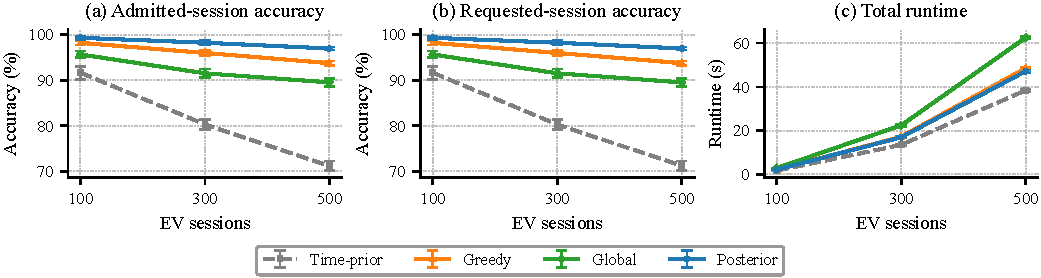
\includegraphics[width=\textwidth,keepaspectratio]{figure3_base_load_comparison.pdf}}
        \caption{\revised{Identification accuracy of the four matchers for admitted and requested sessions as the session load increases from 100 to 500 (95\,\% confidence intervals), and total runtime. Panel (c) is from the full-grid run, which shares the machine with other runs and is therefore slower than the single-cell run reported in TABLE~\ref{table6}.}}
        \label{fig05}
    \end{figure*}

    \begin{table*}[t!]
        \caption{\revised{Accuracy at the representative operating point under identical decision timing (mean over 20 paired repeats; $\pm$ denotes 95\,\% confidence interval; requested-session accuracy equals admitted-session accuracy because no session is blocked). Total runtime is the wall-clock time of one 12-h scenario, measured with the representative cell run alone.}}
        \label{table6}
        \centering
        \begin{tabular}{lcccc}
            \toprule
            \textbf{Matcher} & \revised{\textbf{Admitted-session accuracy}} & \textbf{Requested-session accuracy} & \textbf{90th-percentile decision latency (s)} & \textbf{Total runtime (s)} \\
            \midrule
            Time-prior & \revised{0.712 $\pm$ 0.011} & \revised{0.712} & 416 & \revised{47.7} \\
            Greedy & \revised{0.973 $\pm$ 0.003} & \revised{0.973} & 416 & \revised{57.6} \\
            \revised{\textbf{Global}} & \revised{\textbf{0.999 $\pm$ 0.000}} & \revised{\textbf{0.999}} & 416 & \revised{75.3} \\
            Posterior & \revised{0.984 $\pm$ 0.003} & \revised{0.984} & 416 & \revised{58.0} \\
            \bottomrule
        \end{tabular}
    \end{table*}
    \section{\revised{RESULTS}}

    \revised{This section compares the four matchers inside the shared runtime of Sections~III--V under identical maturity, gating, and finalization timing.}

    \subsection{Base-Load Performance}
    \revised{Waveform evidence lifts identification accuracy far above the timing-only baseline at every evaluated EV-session count, and the prior static cost has the highest mean accuracy of the four matchers (at 100 sessions its difference to the Posterior matcher is not significant; Section~V-B).
    Fig.~\ref{fig05} reports accuracy for $EV \in \{100, 300, 500\}$: the Global matcher reaches $1.000$, $0.999$, and $0.999$, the Posterior matcher $0.998$, $0.991$, and $0.984$, the Greedy matcher $0.996$, $0.989$, and $0.973$, and the time-prior baseline $0.917$, $0.803$, and $0.712$.
    The Posterior matcher is above its greedy base by $+0.011 \pm 0.003$ at 500 sessions; at 100 and 300 sessions the difference ($+0.002 \pm 0.003$) is not detectable at this sample size.

    At $EV = 500$ the misidentification rates are $0.07\,\%$ (Global; 7 of the $10\,000$ decisions), $1.62\,\%$ (Posterior), $2.68\,\%$ (Greedy), and $28.8\,\%$ (Time-prior); TABLE~\ref{table6} lists the accuracies to three decimals.
    The error rates of the waveform costs thus span more than an order of magnitude (the Posterior matcher lowers the Greedy error by $40\,\%$); Section~VI-C traces the spread to whether a cost compares waveform shape or absolute current level.}
    The time-prior baseline reaches \revised{$0.712$} because the candidate-time gate ($\Delta = 120$\,\text{sec}) restricts each EV to an operationally plausible candidate set, so timing alone resolves many cases; the remaining $29\,\%$ is where waveform evidence becomes decisive.

    The accuracy \revised{differences are} obtained under identical decision timing: every matcher uses the same maturity and evaluation-tick rule, so the 90th-percentile decision latency is $416\,\text{sec}$ for all four methods.
    \revised{The latency decomposes as $t_{\text{final},i} - t_{\text{arr},i} = (\hat{t}_{\text{start},i} - t_{\text{arr},i}) + W + d_{\max} + \delta_{\text{tick}}$: the EV-side start-estimate offset (90th percentile $\approx 44$\,\text{sec}), the window $W = 360$\,\text{sec}, the watermark bound $d_{\max} = 10$\,\text{sec}, and the wait for the next 5\,\text{sec} tick ($\delta_{\text{tick}} \leq 4$\,\text{sec}); the identity holds for every traced decision.}
    At $EV = 500$, the Greedy and Posterior matchers have similar total runtimes while the Global matcher is \revised{about 30\,\%} slower (TABLE~\ref{table6})\revised{.}

    \begin{table*}[t!]
        \caption{\revised{Saturation operating points (20 repeats; $\pm$ denotes 95\,\% confidence interval; same runtime, parameters, and seeds as TABLE~\ref{table6}). Each matcher cell lists admitted-session / requested-session accuracy; the latter equals the former times $(1 - \text{blocked ratio})$. The other intervals are at most $0.012$. No fallback path activates and the ground-truth slot is in the candidate set at every decision. S-A: 2\,000 requested sessions on 50 slots; S-B: the 500-session demand on 15 slots with a pool of 15 patterns.}}
        \label{table:saturation}
        \centering
        \scriptsize
        \setlength{\tabcolsep}{3pt}
        \revised{\begin{tabular}{lccccccc}
            \toprule
            \textbf{Point (requested / slots)} & \textbf{Blocked} & \textbf{Cand.} & \textbf{Time-prior} & \textbf{Greedy} & \textbf{Global} & \textbf{Posterior} & \textbf{90th-pct.\ lat.\ (s)} \\
            \midrule
            Base load (500 / 50) & 0.000 & 28.3 & 0.712 / 0.712 & 0.973 / 0.973 & 0.999 / 0.999 & 0.984 $\pm$ 0.003 / 0.984 & 416.0 \\
            S-B (500 / 15) & 0.463 $\pm$ 0.005 & 14.5 & 0.816 / 0.438 & 0.981 / 0.527 & 0.999 / 0.536 & 0.984 $\pm$ 0.005 / 0.528 & 416.9 \\
            S-A (2\,000 / 50) & 0.529 $\pm$ 0.003 & 49.4 & 0.550 / 0.259 & 0.942 / 0.444 & 0.994 / 0.468 & 0.954 $\pm$ 0.004 / 0.450 & 415.6 \\
            \bottomrule
        \end{tabular}}
    \end{table*}

    \revised{\textbf{Saturation operating points.}
    TABLE~\ref{table:saturation} adds two overloaded points on the same runtime, parameters, and seeds: S-A draws $2{,}000$ requested sessions on the 50 slots, and S-B keeps the 500-session demand on 15 slots.
    Blocking occurs for $52.9\,\%$ (S-A) and $46.3\,\%$ (S-B) of the requests, so requested-session accuracy falls to about half of admitted-session accuracy for every matcher (e.g., Global $0.994$ / $0.468$ at S-A).
    On admitted sessions, accuracy follows the candidate-set size rather than the blocking: at S-B ($14.5$ candidates on average) every matcher stays at or above its base-load value, whereas at S-A nearly every decision sees all 50 slots ($49.4$ candidates against $28.3$ at base load), the Posterior and Greedy matchers lose about 3 percentage points (pt), and the timing-only baseline collapses to $0.550$.
    The gate keeps the true slot in every decision and no fallback activates, so the watermark and gating mechanism holds at both overload points; what degrades is discrimination inside larger candidate sets.}

    \revised{\textbf{Static-limit check.}
    In the static setting of~\cite{b14} (300 sessions arriving together on 300 slots, complete 360\,\text{sec} waveforms, no ingestion delay or loss, all slots as candidates, the prior study's codebook; 20 repeats), the prior static cost and the Posterior matcher both identify every pair ($1.000$) when sensing distortion is off, reproducing the $>99\,\%$ of~\cite{b14}.
    With the sensing distortion of Section~V-A on, the prior cost keeps $0.952$, whereas the Posterior and Greedy matchers fall to $0.626$ and $0.581$: the 300 prior patterns differ mainly in current level (closest pairs 1--4\,A apart), which gain and bias blur for the two level-comparing costs; the sensing-on cell also splits the decisions into several batches, so one-to-one assignment no longer spans all 300 pairs (Supplementary Table~S2).
    Because the online and static cells differ in several respects, the gap measures more than the cost of going online.}

    \subsection{Robustness Across Operating Sweeps}

    \revised{The prior static cost stays the most accurate in every sweep except at 5\,\text{sec} EV sampling.}

    \begin{figure}[!t]
        \centerline{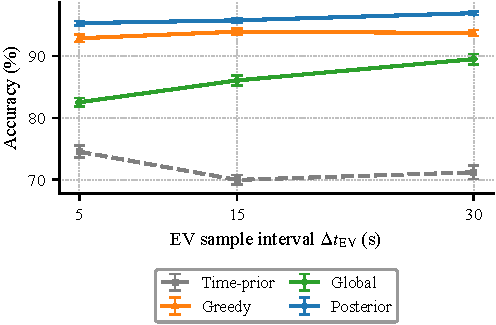
\includegraphics[width=\columnwidth,keepaspectratio]{figure4_sampling_sensitivity.pdf}}
        \caption{\revised{Accuracy of the four matchers across three EV sampling periods at $EV = 500$ ({\unboldmath$d_{\max} = 10$}\,\text{sec}, {\unboldmath$\Delta = 120$}\,\text{sec}; 20 repeats, 95\,\% confidence intervals). The cause of the rise toward coarser {\unboldmath$\Delta t_{\text{EV}}$} is analyzed in the text.}}
        \label{fig06}
    \end{figure}

    \textbf{EV sampling period.}
    \revised{Every waveform cost is less accurate at the densest sampling (Fig.~\ref{fig06}; 3--6\,pt lower at 5\,\text{sec} than at 30\,\text{sec}).
    The Global matcher loses most, so at 5\,\text{sec} the Posterior matcher is the most accurate ($+0.011 \pm 0.006$ against Global, $+0.015 \pm 0.004$ against Greedy).
    Sample noise, the DTW path-length normalization, and the $\sigma_i$ of Eq.~\eqref{eq:pc} are ruled out: the trend persists with the noise removed and with the 5\,\text{sec} samples averaged into 30\,\text{sec} blocks, the refined cost is divided by a fixed number of grid points, and the Greedy matcher, which has no $\sigma_i$, shows the same trend (Supplementary Table~S1).
    The cause is time alignment: each EV-side sample reads the slot current 5--25\,\text{sec} ahead of its timestamp, a fixed offset per session (Section~V-A).
    At 30\,\text{sec} sampling the hold spreads this offset around zero; at 5\,\text{sec} it remains a visible shift that exceeds the $\pm 15$\,\text{sec} DTW band of the Greedy and Posterior costs in about half of the sessions and misaligns the equal-time correlation of the Global cost.
    With the offset fixed at one 5\,\text{sec} sample, every waveform cost recovers to $0.999$ or above and the Posterior--Global difference vanishes (Supplementary Table~S1).
    Dense EV sampling therefore calls for a per-session calibration of the EV-side timestamp offset, whichever cost is used.}

    \textbf{Watermark and candidate margin.}
    Moderate watermark values are sufficient under the present ingestion model.
    At $EV = 500$, the three \revised{waveform} matchers remain stable across $d_{\max} \in \{5, 10, 15\}$\,\text{sec}, with variation \revised{below $0.006$ (no detectable effect at this sample size)}.
    The time-prior baseline stays near $0.70$ over the same range.
    \revised{Across $\Delta \in \{60, 120, 180\}$\,\text{sec} the waveform matchers move by at most 0.6\,pt (Posterior $0.978$, $0.984$, $0.979$).}
    The temporal gate in Eq.~\eqref{eq:e4} retains the ground-truth slot for all admitted sessions in the evaluated envelope ($\approx$28 candidates per EV on average at the representative $\Delta = 120$\,\text{sec}, with no fallback-to-all activations).
    The $\Delta$ sensitivity above therefore reflects matcher discrimination rather than upstream candidate loss.

    \begin{figure*}[!t]
        \centerline{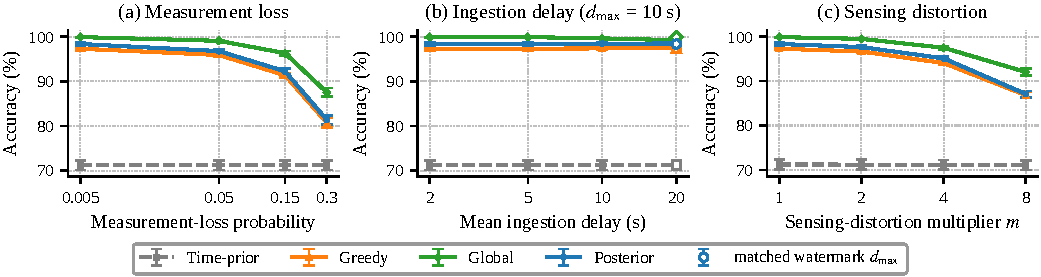
\includegraphics[width=\textwidth,keepaspectratio]{figure7_impairment_sweeps.pdf}}
        \caption{\revised{Accuracy of the four matchers under swept impairments at the representative point ({\unboldmath$EV = 500$}, {\unboldmath$\Delta t_{\text{EV}} = 30$}\,\text{sec}; 20 paired repeats on the TABLE~\ref{table6} seeds; 95\,\% confidence intervals; one factor varied per panel, the others at their defaults). (a) Measurement-loss probability. (b) Mean ingestion delay, with jitter/cap {\unboldmath$1/10$, $2.5/15$, $5/30$, $10/60$}\,\text{sec} and the watermark bound held at {\unboldmath$d_{\max} = 10$}\,\text{sec}; hollow markers: {\unboldmath$d_{\max}$} matched to 60\,\text{sec}. (c) Common multiplier on the sensing-noise, gain, and bias standard deviations of Section~V-A.}}
        \label{fig:impair}
    \end{figure*}

    \revised{\textbf{Ingestion and sensing impairments.}
    Fig.~\ref{fig:impair} sweeps measurement loss, ingestion delay, and sensing distortion for all four matchers; the ordering Global $>$ Posterior $\geq$ Greedy $>$ Time-prior holds in every swept cell.
    Measurement loss hurts most: at 30\,\% loss the Posterior matcher falls from $0.984$ to $0.814$ and the Greedy matcher from $0.973$ to $0.807$, against $0.999$ to $0.875$ for the prior static cost.
    At mean ingestion delays up to 20\,\text{sec} the prior static cost loses only $0.7$\,pt and the other two nothing detectable, because a late measurement is replaced by the last received value and affects at most the end of the window; matching $d_{\max}$ to the 60\,\text{sec} cap removes this loss at 50\,\text{sec} more latency.
    Sensing distortion lowers every waveform cost (at $\times 8$: Global $0.921$, Posterior $0.871$, Greedy $0.869$), and the gap between the Global cost and the other two widens (paired differences, from 1.6 to 5.0\,pt for the Posterior matcher).
    Robustness to sensing distortion is therefore set by what a cost compares (Section~VI-C), whereas loss degrades every waveform cost.}

    \begin{figure}[!t]
        \centerline{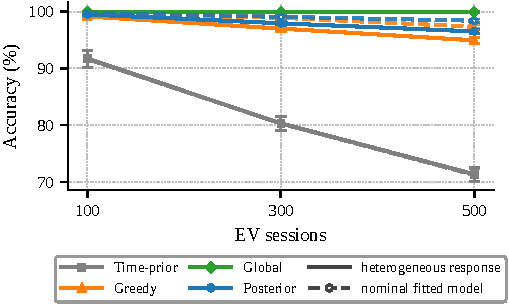
\includegraphics[width=\columnwidth,keepaspectratio]{figure8_heterogeneous_response.pdf}}
        \caption{\revised{Accuracy versus EV-session count under per-session response heterogeneity (first-step lag {\unboldmath$\sim U(2, 30)$}\,\text{sec}, rise rate {\unboldmath$\sim U(1, 10)$}\,A/s; solid lines) and under the nominal fitted model (dashed lines, hollow markers), on the same seeds (only the session dynamics differ); Student-$t$ 95\,\% confidence intervals.}}
        \label{fig:hetero}
    \end{figure}

    \revised{\textbf{Response heterogeneity.}
    Fig.~\ref{fig:hetero} repeats the base-load evaluation with the per-session lag and ramp draws of Section~V-A, keeping arrivals, slots, command patterns, and sensing draws identical.
    The Posterior matcher loses 0.3 / 1.1 / 1.9\,pt (paired differences) at 100 / 300 / 500 sessions ($0.995$ / $0.979$ / $0.965$; the loss at 100 sessions is not detectable at this sample size), the Greedy matcher 2.4\,pt at 500, and the prior static cost nothing detectable ($0.999$); the ordering is unchanged at every session count, and the latency moves by 1\,\text{sec}.
    Over the variation tested, the ordering and the accuracy levels therefore do not depend on the single fitted Wallbox--Tesla response; the matchers compare observed waveforms and need no per-vehicle model.}

    \begin{figure}[!t]
        \centerline{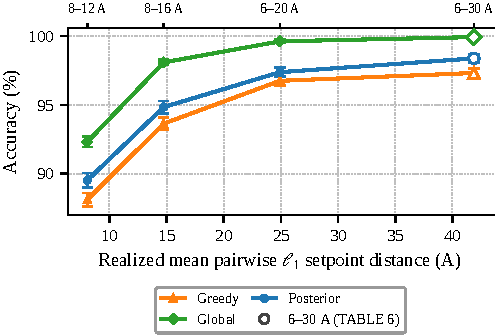
\includegraphics[width=\columnwidth,keepaspectratio]{figure9_codebook_separation.pdf}}
        \caption{\revised{Accuracy versus realized command-codebook separation at the representative point ({\unboldmath$EV = 500$}, 20 paired repeats, 95\,\% confidence intervals), obtained by narrowing the setpoint band of the random codebook (band labels on the upper axis; the hollow 6--30\,A point is the TABLE~\ref{table6} result). The abscissa is the realized mean pairwise {\unboldmath$\ell_1$} setpoint distance.}}
        \label{fig:codebook}
    \end{figure}

    \revised{\textbf{Command-codebook separation.}
    As in all current-modulation identification, the pair is identified through the command modulation rather than through a vehicle signature: response heterogeneity changes accuracy by at most 2.4\,pt (Fig.~\ref{fig:hetero}), whereas accuracy falls as the concurrently issued command patterns become more similar (Fig.~\ref{fig:codebook}).
    Narrowing the setpoint band from 6--30\,A to 6--20, 8--16, and 8--12\,A (mean pairwise $\ell_1$ distance 41.9, 24.9, 14.7, and 8.1\,A), the demand-response case of narrow current bands, lowers all three waveform matchers monotonically with the ordering preserved (Global $0.999 \rightarrow 0.923$, Posterior $0.984 \rightarrow 0.895$, Greedy $0.973 \rightarrow 0.881$), all above the timing-only $0.712$.
    As a design rule within the evaluated envelope, the prior static cost keeps $\geq 0.98$ and the Posterior matcher $\geq 0.94$ while the mean pairwise setpoint distance stays at about 15\,A or more (the 8--16\,A band; Supplementary Section~S6 lists the values per band).}

    \revised{\textbf{Hyperparameter sensitivity.}
    Supplementary Table~S4 varies $\gamma_{\text{prev}}$, $\eta_{\text{mix}}$, and $\beta_{\text{curr}}$ one at a time over five values around their TABLE~\ref{table:hyper} values on the evaluation repeats of the representative point.
    All fifteen settings lie in $0.9815$--$0.9838$, above the Greedy reference ($0.973$) and below the Global reference ($0.999$); $\eta_{\text{mix}}$ and $\beta_{\text{curr}}$ change the result by at most $0.0002$ and $\gamma_{\text{prev}}$ by at most $0.0023$.
    The Posterior matcher's results, including its gain over single-prefix scoring, therefore depend little on these three settings.}



    \subsection{\revised{Failure Analysis and} Ablation}

    \begin{table}[htbp]
        \caption{\revised{Failure taxonomy of the Posterior matcher at the representative point (20 evaluation repeats; 10\,000 decisions, 162 misidentifications). One primary class per error, assigned in the listed order; ``exposed'' is the number of decisions in which the condition is present, and the classes record co-occurrence rather than established cause.}}
        \label{table:taxonomy}
        \centering
        \scriptsize
        \setlength{\tabcolsep}{3pt}
        \revised{\begin{tabular}{@{}lrrrr@{}}
            \toprule
            \textbf{Breakdown} & \textbf{Exposed} & \textbf{Errors} & \textbf{Cond. rate} & \textbf{Share} \\
            \midrule
            Truncated window ($t_{\text{eff}} - \hat{t}_{\text{start}} < W$) & 0 & 0 & -- & 0\,\% \\
            Leading sample missing at the decision tick & 61 & 2 & 3.3\,\% & 1.2\,\% \\
            Sensing draw beyond threshold & 3\,411 & 61 & 1.8\,\% & 37.7\,\% \\
            Step-signature overlap (remainder) & 10\,000 & 99 & 1.0\,\% & 61.1\,\% \\
            \midrule
            Candidate set $\leq 10$ & 110 & 0 & 0.0\,\% & 0.0\,\% \\
            Candidate set 11--25 & 2\,795 & 32 & 1.1\,\% & 19.8\,\% \\
            Candidate set 26--40 & 6\,995 & 126 & 1.8\,\% & 77.8\,\% \\
            Candidate set $> 40$ & 100 & 4 & 4.0\,\% & 2.5\,\% \\
            \midrule
            All decisions & 10\,000 & 162 & 1.62\,\% & 100\,\% \\
            \bottomrule
        \end{tabular}}
    \end{table}

    \revised{\textbf{Failure taxonomy.}} Residual error stems from candidate-set ambiguity rather than from runtime-timing pathologies.
    \revised{TABLE~\ref{table:taxonomy} breaks down the 162 misidentifications of the Posterior matcher among the $10{,}000$ decisions at the representative point, from full decision traces.
    No error involves a truncated window, because every session lasts at least $W$ and all six command steps are observed; 2 errors (1.2\,\%) coincide with a leading sample still missing at the decision tick (a lost measurement, not a late one, since $d_{\max}$ equals the delay cap), 61 (37.7\,\%) with a sensing draw beyond $2\sigma$ or a large read offset (53 of them the offset), and the remaining 99 (61.1\,\%) are confusions between two gated candidates with none of these conditions (Supplementary Section~S6 bins them by command-pattern distance).
    The error rate rises with candidate-set size, from 0\,\% ($\leq 10$ candidates) to 4.0\,\% ($> 40$), while the true slot is inside the candidate set in every decision.
    At the same point the Greedy matcher makes 268 errors and the prior static cost 7, and 43\,\% of the Posterior matcher's errors are near-ties with a posterior gap below $0.05$; Supplementary Fig.~S1 shows how the beliefs of the two leading candidates separate within one decision.}

    \begin{figure*}[!t]
        \centerline{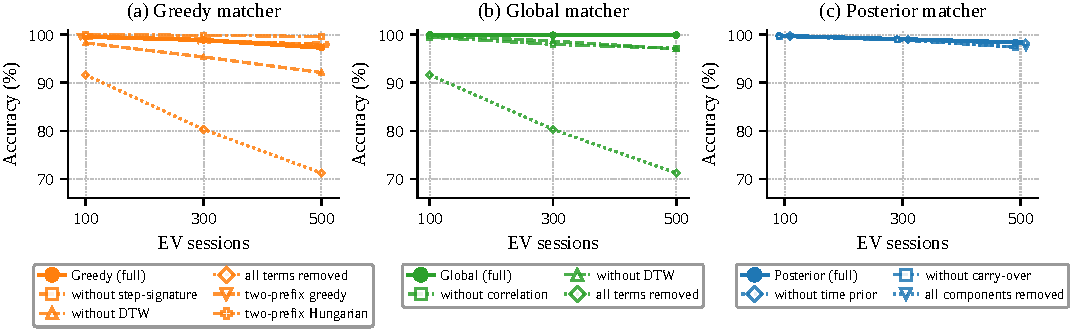
\includegraphics[width=\textwidth]{figure6_ablation_summary.pdf}}
        \caption{\revised{Ablation results for the three matcher families, computed on the evaluation repeats of TABLE~\ref{table:calib_eval} (20 paired repeats at {\unboldmath$EV \in \{100, 500\}$}, 15 held-out repeats at {\unboldmath$EV{\,}={\,}300$}). Open markers in the Greedy panel: the stateless two-prefix variant of Eq.~\eqref{eq:twoprefix} (greedy and Hungarian assignment identical). Markers of overlapping curves are offset horizontally for visibility.}}
        \label{fig08}
    \end{figure*}

    \begin{table}[htbp]
        \caption{\revised{Two-prefix ablation of the Posterior matcher (Eq.~\eqref{eq:twoprefix}) on the base-load seeds (mean $\pm$ Student-$t$ 95\,\% confidence interval; paired differences on identical scenarios). Greedy and Hungarian assignment give identical accuracy in every cell.}}
        \label{table:twoprefix}
        \centering
        \scriptsize
        \setlength{\tabcolsep}{2pt}
        \revised{\begin{tabular}{@{}l@{\hspace{4pt}}ccc@{}}
            \toprule
            \textbf{Variant} & \textbf{EV 100} & \textbf{EV 300} & \textbf{EV 500} \\
            \midrule
            Greedy (single prefix) & 0.996 & 0.989 & 0.973 \\
            Posterior, no carry-over & 0.997 & 0.989 & 0.974 \\
            Two-prefix (greedy = Hung.) & 0.996 $\pm$ 0.003 & 0.988 $\pm$ 0.003 & 0.980 $\pm$ 0.003 \\
            Posterior (full) & 0.998 & 0.991 & 0.984 \\
            \midrule
            Posterior $-$ two-prefix & $+$0.002 $\pm$ 0.002 & $+$0.002 $\pm$ 0.002 & $+$0.004 $\pm$ 0.002 \\
            Two-prefix $-$ Greedy & $+$0.000 $\pm$ 0.003 & $-$0.001 $\pm$ 0.004 & $+$0.007 $\pm$ 0.004 \\
            \bottomrule
        \end{tabular}}
    \end{table}

    \revised{\textbf{Component ablation and the two-prefix variant.}} Ablation identifies the components responsible for the observed behavior (Fig.~\ref{fig08})\revised{.
    For the Greedy matcher, removing the step-signature term raises accuracy at $EV = 500$ from $0.973$ to $0.996$, removing DTW lowers it to $0.921$, and removing both leaves the timing-only cost ($0.712$).
    For the Global matcher the full score is strongest ($0.999$; $0.972$ without correlation, $0.970$ without DTW).
    For the Posterior matcher, removing the within-decision carry-over returns accuracy to the greedy level ($0.974$), and removing the shaped time prior has no detectable effect at this sample size ($0.983$).
    Removing the carry-over, however, also removes the only path by which the 60\,\% prefix reaches the decision.
    To separate the two effects, a stateless two-prefix variant simply averages the waveform cost of Eqs.~\eqref{eq:e6}--\eqref{eq:e7} over the same two prefixes,
    \begin{equation}\label{eq:twoprefix}
        c^{(2p)}_{i,s} = \tfrac{1}{2}\left(c^{60\%}_{i,s} + c^{100\%}_{i,s}\right),
    \end{equation}
    with no time prior and no posterior state, and is assigned greedily or by the Hungarian method (TABLE~\ref{table:twoprefix}; open markers in Fig.~\ref{fig08}).
    At 500 sessions the Posterior matcher's 1.1\,pt gain over the Greedy matcher thus splits into $+0.7 \pm 0.4$\,pt from also scoring the 60\,\% prefix and $+0.4 \pm 0.2$\,pt from combining both prefixes through the posterior; at 100 and 300 sessions no difference among the variants is detectable at this sample size.
    Most of the gain is therefore multi-prefix evidence, with a small posterior increment at the largest load.}

    \revised{\textbf{Cost-term partition.}
    Removing one term at a time on the sensing axis of Fig.~\ref{fig:impair}(c) (Supplementary Table~S3), the banded DTW cost alone reaches $0.996$ at base load and $0.992$ at sensing $\times 8$, whereas the step term alone falls to $0.743$ and the Global matcher without its correlation term to $0.535$.
    This explains the spread seen in Section~VI-A: the level-comparing terms (the per-step term and the raw-current DTW of the Global cost) are what gain and bias break, while the correlation and z-normalized DTW terms, which ignore gain and bias, lose less than 1\,pt.
    The frozen costs of TABLE~\ref{table:hyper} are kept, since adopting the DTW-only variant would mean tuning on the evaluation slice.}
    \section{\revised{DISCUSSION: LIMITATIONS, DEPLOYMENT, AND SECURITY}}

    \subsection{\revised{Simulation-to-Deployment Gap}}
    \revised{The evaluation is simulation-based (one site, one fitted Wallbox--Tesla response, independent per-measurement delay and loss, a random codebook); its waveforms are measurement-derived, but the ingestion parameters, the sensing-distortion magnitudes, and the codebook are assumptions.
    The sweeps bound the loss from each deviation: delay up to a 20\,\text{sec} mean costs at most 0.7\,pt, whereas measurement loss, sensing distortion, and narrow codebooks degrade every waveform cost (Figs.~\ref{fig:impair} and~\ref{fig:codebook}).
    The simulation cannot supply the joint behavior of these impairments on an operational network, where a congested cellular uplink or a large cloud broker produces correlated bursts of delay and loss, nor other vehicle models.
    A deployment therefore needs measured delay quantiles per site to place $d_{\max}$, measured loss rates, a per-model sensing calibration, a per-session timestamp-offset calibration when EV sampling is dense, and a codebook matched to the site's current bands.}

    \subsection{\revised{Scalability and Congestion}}
    \revised{The computing time of one decision grows with the candidate count $|C_i|$, not with the site size, because the assignment is solved only over the few sessions maturing at the same tick; $|C_i|$ averages about 6, 17, and 28 at 100, 300, and 500 sessions.
    Multi-site aggregation is the simpler direction: if each EV stream can be attributed to a site (e.g., by the network's site identifier), the gate admits only that site's slots, so sites are independent copies of the runtime and scale linearly.
    Larger single sites are harder: at 2\,000 sessions on 50 slots the prior static cost keeps $0.994$ while the other two waveform costs lose about 3\,pt (TABLE~\ref{table:saturation}).
    Hundreds of simultaneously active sessions on one site would thus need a hierarchical gate (by feeder or sub-site) that keeps $|C_i|$ in the tens, which was not evaluated.
    Under congestion, requested-session accuracy is the meaningful figure; it is below $0.5$ for every matcher at S-A because more than half of the requests are blocked.}

    \subsection{\revised{Candidate Gating and Watermark Strategy}}
    \revised{If the gate's exclusion of the true slot (Section~III-C) empties the candidate set, the runtime falls back to all slots and logs the event; if other slots remain, the true slot cannot be selected.
    Neither case occurs in the evaluated envelope (TABLES~\ref{table:saturation} and~\ref{table:taxonomy}), so a deployment should monitor the share of empty candidate sets and the start-estimate offsets (90th percentile $\approx 44$\,\text{sec} here); near-tie decisions ($43\,\%$ of the Posterior matcher's errors have a posterior gap below $0.05$) could also be sent to a confirmation path, a safeguard not evaluated here.
    An adaptive watermark bound would set $d_{\max}$ per session from measured delay quantiles (e.g., a running 99th percentile of the MeterValues arrival lag), gaining exactness for late tails at the price of latency, since $d_{\max}$ adds directly to the decision latency.
    In the sweeps the fixed bound costs at most $0.7$\,pt (the prior static cost at a 20\,\text{sec} mean delay), which a 60\,\text{sec} bound recovers at 50\,\text{sec} more latency (Fig.~\ref{fig:impair}(b)).}

    \subsection{\revised{Operational Side-Effects of Current Modulation and Protocol Coexistence}}
    \revised{The modulation only lowers the allowable current within the operator's range, and only until the pair is finalized (416\,\text{sec} after arrival at the 90th percentile, at most 464\,\text{sec}); the port then returns to its normal limit.
    With the 6--30\,A codebook (mean setpoint $\approx 15$\,A) under a 30\,A limit, the charge withheld up to the 90th-percentile decision time is $\approx 1.7$\,A$\cdot$h per phase, about 1\,\% of a 40\,kWh battery at 230\,V (at most 3.5\,A$\cdot$h, about 2\,\%, if every step were 0\,A); it is delivered later rather than lost, delaying a given state of charge by at most the modulated time (under 8\,min).
    An IEC~61851-1 charger conveys only a maximum allowable current through the control pilot, so the on-board charger follows a lower limit exactly as under smart-charging curtailment, and the battery management system keeps full authority over the battery.
    No setpoint exceeds the operator's limit, so site current stays at or below that of constant-limit charging, and the steps (at most 30\,A per port every 60\,\text{sec}) are slow setpoint changes of the kind smart charging already issues, not fast battery cycling, apart from the 0\,A first step discussed below.
    Two points remain for deployment: some vehicles may pause when the allowable current is set to 0\,A in the first step, which must be checked per model, and stopping the modulation after finalization was not simulated (the simulator re-issues the pattern).
    Where ISO~15118 plug-and-charge is available on both sides, the identity is transmitted and no modulation is needed; the framework complements such protocols by covering the legacy IEC~61851 fleet, by cross-checking vehicle-side telemetry against charger-side records, and by requiring no hardware change, so it can be retired port by port.}

    \subsection{\revised{Security Sensitivity}}
    \revised{(i)~Spoofing: a fabricated EV stream must reproduce the command pattern of the slot it claims, and patterns are drawn per session from a seeded pool known only to the backend, so a stream prepared in advance does not match the live command; a spoofed stream that still wins a slot displaces the legitimate session only within the same batch, and across batches both can be finalized to the same slot, which the runtime does not prevent but the backend can see and count (duplicate claims also arise from ordinary misidentification, so their count is a useful monitoring signal).
    (ii)~Timestamp manipulation: records after the watermark are ignored, and a stream shifted by more than $\Delta$ from every active slot leaves an empty, logged candidate set, but a shift into another slot's active interval is neither detected nor authenticated.
    (iii)~Replay: patterns are reused from a pool of fifty, so a replay that coincides with a live re-issue of its pattern is not resisted.
    Nor does the design resist a compromised control plane or real-time synthesis of the live command by an attacker at the port; a quantitative evaluation is future work.}

    \section{CONCLUSION}
    \looseness=1 This paper extended the measurement-based Wallbox--Tesla current-generation model of prior MCCT work~\cite{b14} into an event-driven online runtime, in which EV sessions arrive and depart asynchronously and EV-side observations reach the backend as delayed \revised{slot-unlabeled} telemetry.
    Unlike static batch assignment over completed waveforms, the resulting decision problem requires irrevocable finalization from a maturing prefix of EV-side evidence under a watermark-governed maturity rule and time-tolerance candidate gating.
    \revised{The proposed runtime decided every admitted session at a bounded latency with the true slot among its candidates, even under overload, so that the matching algorithms could be compared under identical decision timing.
    In the representative 500-session scenario, waveform evidence raised identification accuracy from 0.712 for the timing-only baseline to 0.973 for the greedy waveform cost, 0.984 for the two-stage posterior matcher, and 0.999 for the prior static correlation--DTW cost, which stayed the most accurate at the saturation points and in every sweep except the densest EV sampling, where a per-session timestamp offset of the EV sensor degrades it most.
    Ablation and a term partition trace these differences to what each cost compares: correlation ignores the per-session gain and bias of the EV sensor, whereas a per-step comparison of current levels does not, and the posterior matcher's gain of 1.1\,pt over its greedy base comes mostly from also scoring the 60\,\% prefix.
    Extending current-modulation identification to cloud-connected legacy AC operation therefore requires online finalization of delayed evidence within a gated candidate set, a matching cost that is robust to sensor gain and bias, and command patterns separated by a mean pairwise setpoint distance of about 15\,A or more, which within the evaluated envelope keeps the prior cost at 0.98 or above; measurement loss and sensing distortion set the remaining budgets.
    Future work should address field measurement of delay and loss, per-model response data, per-session offset calibration, adaptive watermarks, hierarchical gating for very large sites, a quantitative security evaluation, and stopping rules for early finalization.}

    \section*{CODE AVAILABILITY}
    The source code used in this study is publicly available \revised{in~\cite{bcode}}; the repository contains the event-driven simulator, the four matcher implementations, the per-repeat random seeds, and the \revised{\mbox{reproduce\_all}} driver script that regenerates \revised{the tables and figures of Section~VI. The Supplementary Material (Tables~S1--S4, Fig.~S1, and Section~S6) is included in the same repository.}

    \section*{ACKNOWLEDGMENT}
    The formulation reuses the charging-current generation model of Nomura~\textit{et al.}~\cite{b14}; the EV-side response-lag settings are treated as waveform-generation delays informed by the FAT measurements reported by Imanaka and Baba~\cite{bimanaka25}, while backend telemetry ingestion is modeled separately. The original MCCT proposal by Baba and Imanaka~\cite{b13} is acknowledged as the conceptual origin of this line of work.

    \begingroup
    \scriptsize
    \sloppy
    \emergencystretch=2em
    \tolerance=3000
    \hbadness=10000
    \begin{thebibliography}{42}
    \setlength{\itemsep}{0pt}\setlength{\parsep}{0pt}\setlength{\parskip}{0pt}
                \bibitem{biea26} International Energy Agency, \textit{Global EV Outlook 2026}, Paris, France, 2026. [Online]. Available: \url{https://www.iea.org/reports/global-ev-outlook-2026}

        \bibitem{b2} F. Ahmed, S. Ahmad, M. T. Rahman, M. R. Hazari, R. Faiz, T. Ahmed, and M. Karimi, ``A holistic review of electric vehicle charging impacts on power distribution networks: Technical challenges, smart mitigation strategies and future directions,'' \textit{Appl. Energy}, vol.~402, art.~no.~126961, 2026, doi:~10.1016/j.apenergy.2025.126961.

        \bibitem{b3} S. Powell, G. V. Cezar, L. Min, I. M. L. Azevedo, and R. Rajagopal, ``Charging infrastructure access and operation to reduce the grid impacts of deep electric vehicle adoption,'' \textit{Nat. Energy}, vol.~7, no.~10, pp.~932--945, Oct.~2022.

        \bibitem{b5} P. V. Dahiwale, Z. H. Rather, and I. Mitra, ``A comprehensive review of smart charging strategies for electric vehicles and way forward,'' \textit{IEEE Trans. Intell. Transp. Syst.}, vol.~25, no.~9, pp.~10462--10482, Sep.~2024, doi:~10.1109/TITS.2024.3365581.

        \bibitem{b8} S. S. G. Acharige, M. E. Haque, M. T. Arif, N. Hosseinzadeh, K. N. Hasan, and A. M. T. Oo, ``Review of electric vehicle charging technologies, standards, architectures, and converter configurations,'' \textit{IEEE Access}, vol.~11, pp.~41218--41255, 2023.

        \bibitem{biec} \revised{International Electrotechnical Commission, \textit{IEC 61851-1:2017, Electric Vehicle Conductive Charging System --- Part 1: General Requirements}, ed.~3.0, Geneva, Switzerland, Feb.~2017.}

        \bibitem{b6} H. S. Das, M. M. Rahman, S. Li, and C. W. Tan, ``Electric vehicles standards, charging infrastructure, and impact on grid integration: A technological review,'' \textit{Renew. Sustain. Energy Rev.}, vol.~120, art.~no.~109618, Mar.~2020.

        \bibitem{b7} International Organization for Standardization, \textit{ISO 15118-20:2022, Road Vehicles --- Vehicle to Grid Communication Interface --- Part 20: \revised{2nd Generation Network Layer and Application Layer Requirements}}, Geneva, Switzerland, 2022.

        \bibitem{b13} H. Baba and M. Imanaka, ``Report on basic experiments of normal charger-EV linking technology,'' in \textit{Proc. IEEJ EIS Division Conf.}, \revised{Higashiosaka, Japan,} Paper GS8-6, \revised{Sep.}~2024.

        \bibitem{b14} N. Nomura, M. Imanaka, H. Baba, and D. Kodaira, ``Individual identification of multiple EV--charger pairs via modulated charging current technology,'' in \textit{Proc. 14th Int. Conf. Renewable Energy Research and Applications (ICRERA)}, Vienna, Austria, Oct.~2025, pp.~246--251, doi:~10.1109/ICRERA66237.2025.11283721.

        \bibitem{b15} H. W. Kuhn, ``The Hungarian method for the assignment problem,'' \textit{Naval Res. Logist. Quart.}, vol.~2, no.~1--2, pp.~83--97, 1955.

        \bibitem{b26} T. Akidau \textit{et al.}, ``The Dataflow model: A practical approach to balancing correctness, latency, and cost in massive-scale, unbounded, out-of-order data processing,'' \textit{Proc. VLDB Endow.}, vol.~8, no.~12, pp.~1792--1803, 2015.

        \bibitem{bhart} G. W. Hart, ``Nonintrusive appliance load monitoring,'' \textit{Proc. IEEE}, vol.~80, no.~12, pp.~1870--1891, Dec.~1992.

        \bibitem{b9} A. M. A. Haidar and K. M. Muttaqi, ``Behavioral characterization of electric vehicle charging loads in a distribution power grid through modeling of battery chargers,'' \textit{IEEE Trans. Ind. Appl.}, vol.~52, no.~1, pp.~483--492, Jan.--Feb.~2016, doi:~10.1109/TIA.2015.2483705.

        \bibitem{b10} F. Ferretti and A. De~Paola, ``Machine learning identification of electric vehicles from charging session data,'' \textit{Energy AI}, vol.~20, art.~no.~100502, May~2025, doi:~10.1016/j.egyai.2025.100502.

        \bibitem{b11} A. Brighente, M. Conti, D. Donadel, and F. Turrin, ``EVScout2.0: Electric vehicle profiling through charging profile,'' \textit{ACM Trans. Cyber-Phys. Syst.}, vol.~8, no.~2, art.~no.~11, Apr.~2024, doi:~10.1145/3565268.

        \bibitem{b12} S. Matrone, E. G. C. Ogliari, A. Nespoli, G. Gruosso, and A. Gandelli, ``Electric vehicles charging sessions classification technique for optimized battery charge based on machine learning,'' \textit{IEEE Access}, vol.~11, pp.~52444--52451, 2023.

        \bibitem{bmarchiori25} F. Marchiori, D. Donadel, A. Brighente, and M. Conti, ``Profiling electric vehicles via early charging voltage patterns,'' presented at the \textit{AI \& CPSS Workshop, Int. Conf. Availability, Reliability and Security (ARES)}, Ghent, Belgium, Aug.~2025. [Online]. Available: \url{https://arxiv.org/abs/2506.07714}

        \bibitem{bferretti24} F. Ferretti, A. De~Paola, H. Scholz, S. Tarantola, and E. Kotsakis, ``Reference power tracking for AC charging of electric vehicles,'' \textit{IEEE Access}, vol.~12, pp.~174245--174254, 2024, doi:~10.1109/ACCESS.2024.3501474.

        \bibitem{b20} W. Kim, P.-Y. Lee, J. Kim, and K.-S. Kim, ``A robust state of charge estimation approach based on nonlinear battery cell model for lithium-ion batteries in electric vehicles,'' \textit{IEEE Trans. Veh. Technol.}, vol.~70, no.~6, pp.~5638--5647, Jun.~2021, doi:~10.1109/TVT.2021.3079934.

        \bibitem{b21} M. Pasetti, S. Dello~Iacono, and D. Zaninelli, ``Real-time state of charge estimation of light electric vehicles based on active power consumption,'' \textit{IEEE Access}, vol.~11, pp.~110995--111010, 2023, doi:~10.1109/ACCESS.2023.3322651.

        \bibitem{bjameel24} \revised{S. M. Jameel, J. M. Altmemi, A. A. Oglah, M. A. Abbas, and A. H. Sabry, ``Predicting batteries second-life state-of-health with first-life data and on-board voltage measurements using support vector regression,'' \textit{J. Energy Storage}, vol.~104, art.~no.~114554, Dec.~2024, doi:~10.1016/j.est.2024.114554.}

        \bibitem{bkhanda} A. Khanda, A. Satpathy, and S. K. Das, ``SMART-CHARGE: Stable matching algorithm for electric vehicle charging in subscription-based models,'' \textit{Pervasive Mobile Comput.}, vol.~118, art.~no.~102197, May~2026, doi:~10.1016/j.pmcj.2026.102197.

        \bibitem{breactttc} A. Satpathy, A. Khanda, C. Swain, and S. K. Das, ``ReACT-TTC: Capacity-aware top trading cycles for post-choice reassignment in shared CPS,'' presented at the \textit{17th ACM/IEEE Int. Conf. Cyber-Physical Syst. (ICCPS)}, Saint-Malo, France, May~2026. [Online]. Available: \url{https://arxiv.org/abs/2602.00859}, doi:~10.48550/arXiv.2602.00859.

        \bibitem{b17} R. M. Karp, U. V. Vazirani, and V. V. Vazirani, ``An optimal algorithm for on-line bipartite matching,'' in \textit{Proc. 22nd ACM Symp. Theory of Computing (STOC)}, 1990, pp.~352--358.

        \bibitem{b18} A. Mehta, ``Online matching and ad allocation,'' \textit{Found. Trends Theor. Comput. Sci.}, vol.~8, no.~4, pp.~265--368, 2013.

        \bibitem{bemek16} Y. Emek, S. Kutten, and R. Wattenhofer, ``Online matching: Haste makes waste!,'' in \textit{Proc. 48th Annu. ACM Symp. Theory Comput. (STOC)}, Cambridge, MA, USA, Jun.~2016, pp.~333--344, doi:~10.1145/2897518.2897557.

        \bibitem{b19} Y. Bar-Shalom, X. R. Li, and T. Kirubarajan, \textit{Estimation with Applications to Tracking and Navigation}. New York, NY, USA: Wiley, 2001.

        \bibitem{bsarkka} S. S\"{a}rkk\"{a}, \textit{Bayesian Filtering and Smoothing}. Cambridge, U.K.: Cambridge Univ. Press, 2013.

        \bibitem{bsabry17} \revised{A. H. Sabry, W. Z. W. Hasan, M. Z. A. Ab. Kadir, M. A. M. Radzi, and S. Shafie, ``DC-based smart PV-powered home energy management system based on voltage matching and RF module,'' \textit{PLoS ONE}, vol.~12, no.~9, art.~no.~e0185012, Sep.~2017, doi:~10.1371/journal.pone.0185012.}
        \bibitem{b22} Open Charge Alliance, \textit{Open Charge Point Protocol 2.0.1, Part~2 --- Specification}, Arnhem, The Netherlands, 2020. [Online]. Available: \revised{\urlocpp}

        \bibitem{b23} I. Fette and A. Melnikov, ``The WebSocket Protocol,'' Internet Engineering Task Force, RFC~6455, Dec.~2011.

        \bibitem{b24} V. Paxson, M. Allman, J. Chu, and M. Sargent, ``Computing TCP's Retransmission Timer,'' Internet Engineering Task Force, RFC~6298, Jun.~2011.

        \bibitem{b25} Federal Communications Commission, \textit{Measuring Fixed Broadband---Thirteenth Report}, Washington, DC, USA, Aug.~2024. [Online]. Available: \url{https://www.fcc.gov/reports-research/reports/measuring-broadband-america/measuring-fixed-broadband-thirteenth-report}

        \bibitem{bimanaka23} M. Imanaka, Y. Ishida, H. Baba, and W. Hirohashi, ``Prototyping reference model for combined behavior of ICT systems and energy equipment'' (in Japanese), \textit{Seisan-Kenkyu (J. Inst. Industrial Sci., Univ. of Tokyo)}, vol.~75, no.~4, pp.~333--341, 2023.

        \bibitem{bsatya} M. Satyanarayanan, ``The emergence of edge computing,'' \textit{Computer}, vol.~50, no.~1, pp.~30--39, Jan.~2017.

        \bibitem{b16} H. Sakoe and S. Chiba, ``Dynamic programming algorithm optimization for spoken word recognition,'' \textit{IEEE Trans. Acoust., Speech, Signal Process.}, vol.~26, no.~1, pp.~43--49, 1978.

        \bibitem{bbakirci23} \revised{M. Bakirci, ``Data-driven system identification of a modified differential drive mobile robot through on-plane motion tests,'' \textit{Electrica}, vol.~23, no.~3, pp.~619--633, Aug.~2023, doi:~10.5152/electrica.2023.22164.}
        \bibitem{bimanaka25} M. Imanaka and H. Baba, ``Measurement of both full activation time and ICT response time for fast demand response of electric vehicle charging,'' \textit{IEEJ Trans. Electr. Electron. Eng.}, vol.~21, no.~2, pp.~307--315, Feb.~2026, doi:~10.1002/tee.70176.

        \bibitem{bzaptec} Zaptec, \textit{Zaptec Go2 OCPP 1.6J Supported Configuration Keys}. [Online]. Available: \url{https://docs.zaptec.com/docs/zaptec-go2-ocpp-16j-supported-configuration-keys}

        \bibitem{babb} \revised{ABB, \textit{Terra AC Wallbox --- OCPP 1.6 Implementation Overview}, v1.8 (firmware 1.6.6), May~2023. [Online]. Available: \urlabb}

        \bibitem{bcode} \revised{J. Yang and D. Kodaira, ``Watermark-based online EV--charger matching from delayed slot-unlabeled telemetry: Source code and reproduction scripts,'' GitHub repository, 2026. [Online]. Available: {\def\UrlBreakPenalty{100}\def\UrlBigBreakPenalty{100}\urlrepo}}

\end{thebibliography}
    \endgroup

    \begin{IEEEbiography}[{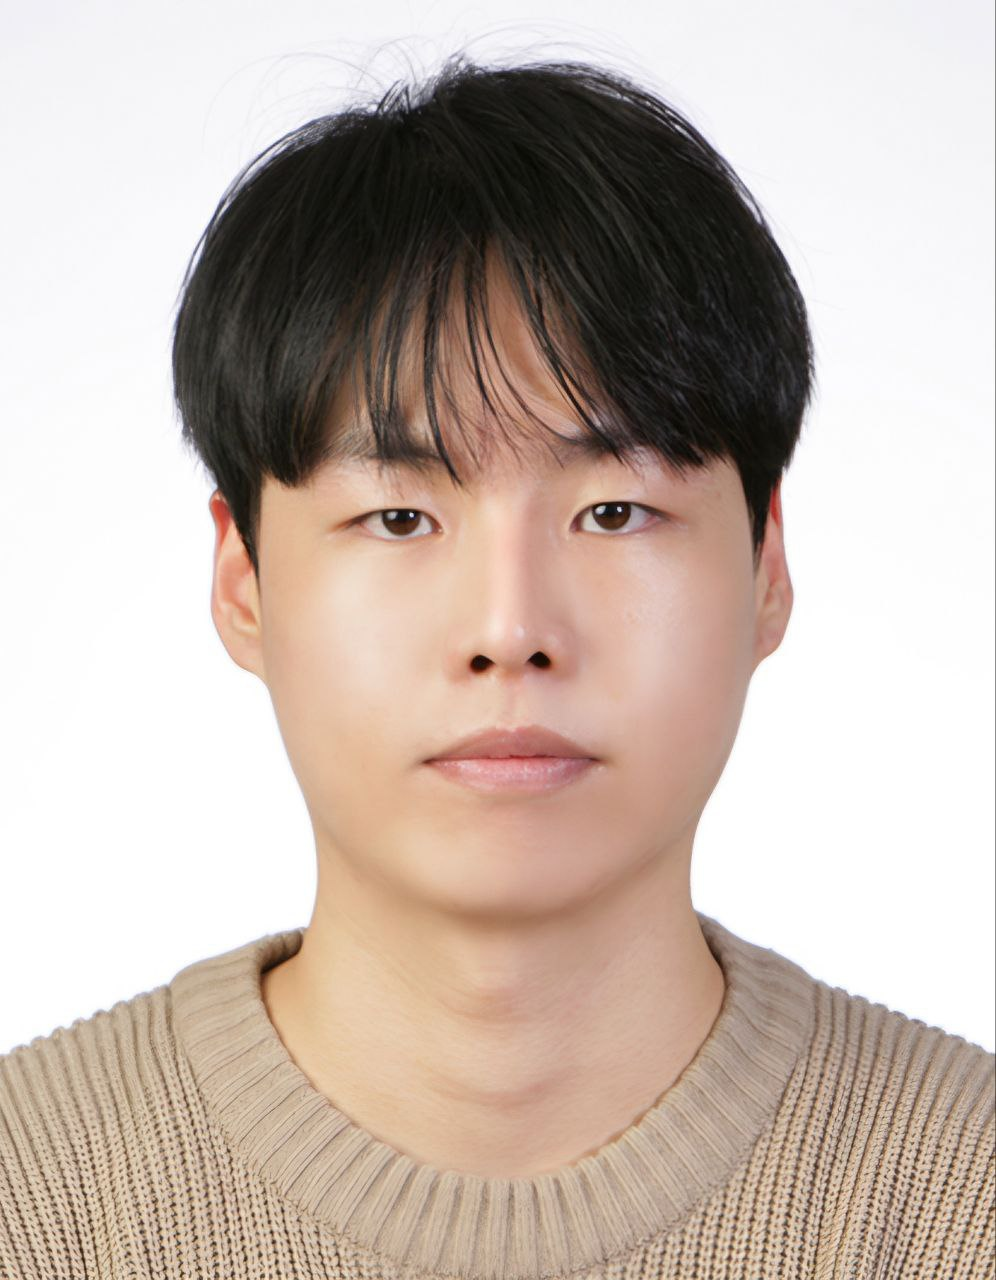
\includegraphics[width=1in,height=1.25in,clip,keepaspectratio]{author1_yang.png}}]{Jiseok Yang} received the B.S.\ degree in electrical and electronic engineering from Chungbuk National University, Cheongju, South Korea, in 2025. He is currently pursuing the M.S.\ degree in systems and information engineering with the University of Tsukuba, Japan. His research interests include EV charging, asynchronous cloud telemetry, and online matching and identification for cyber-physical systems, with a current focus on Bayesian posterior tracking under partial and delayed observability.
    \end{IEEEbiography}
    \begin{IEEEbiography}[{
\includegraphics[width=1in,height=1.25in,clip,keepaspectratio]{author2_kodaira.png}}]{Daisuke Kodaira} (Member,~IEEE) received the Ph.D.\ degree in electrical engineering from Tokyo Metropolitan University, Japan. He is an Associate Professor with the Institute of Systems and Information Engineering, University of Tsukuba, Japan, with research interests in intelligent transportation systems, mobility-data platforms, EV charging infrastructure, and cyber-physical integration.
    \end{IEEEbiography}

    \EOD

\end{document}
